%  MDPI Algorithms submission. Built from the shared section sources by eaagn/to_mdpi.py;
%DIF LATEXDIFF DIFFERENCE FILE
%DIF DEL ../revision/submitted_v1/main.tex   Wed Nov 25 16:49:39 2026
%DIF ADD main.tex                            Thu Nov 26 23:23:23 2026
%  numbers are filled from paper/numbers.json by eaagn/render.py.
%=================================================================
\documentclass[algorithms,article,submit,pdftex,oneauthor]{Definitions/mdpi}

%=================================================================
% MDPI internal commands - do not modify
\firstpage{1}
\makeatletter
\setcounter{page}{\@firstpage}
\makeatother
\pubvolume{1}
\issuenum{1}
\articlenumber{0}
\pubyear{2026}
\copyrightyear{2026}
\datereceived{ }
\daterevised{ }
\dateaccepted{ }
\datepublished{ }

%=================================================================
% Packages and commands (most packages are loaded by the MDPI class)
\newcommand{\U}{\mathcal{U}}
\newcommand{\B}{\mathcal{B}}
\newif\ifgg
\ggtrue


%=================================================================
\Title{Event-Aware AGN-Net: Learning Which Graph Updates Can Be Skipped in Streaming Respiratory Sound Event Detection}

\Author{Md. Redwan Islam}

\AuthorNames{Md. Redwan Islam}

\address{School of Computing, University of Georgia, Athens, GA 30602, USA; MdRedwan.Islam@uga.edu}


%DIF 40c40
%DIF < \abstract{Continuous auscultation needs streaming detectors that observe all audio without recomputing expensive internal representations at every step, but existing selective-update methods skip work based on input or representation change or on learned gates, and none of them estimates which skipped updates matter. We propose Event-Aware AGN-Net, a streaming respiratory sound event detector that keeps a persistent graph of 64 frequency regions and updates the region states only on a budget-limited set chosen by a lightweight controller. The controller is trained on a counterfactual skip-harm utility: the change in the model's output when a region's update is withheld. On the SPRSound paediatric benchmark (three seeds, patient-level bootstrap), with 25\% of the graph updates the controller preserves the full-update model's detections with an event-preservation F-score of 0.78, compared with 0.56 for a change-prediction objective and 0.41 for random selection. The gain holds in every seed and on a later data release, and the event F-score against the annotations is non-inferior to full updating. The advantage carries over to a graph gated recurrent unit (GRU) cell, while the end-to-end speedup is modest (1.14-fold). Predicting the task consequence of skipping, rather than representation change, lets streaming biomedical models decide which updates to compute.
%DIF -------
\abstract{Continuous auscultation needs streaming detectors that observe all audio without recomputing expensive internal representations at every step\DIFdelbegin \DIFdel{, but existing }\DIFdelend \DIFaddbegin \DIFadd{. Existing }\DIFaddend selective-update methods skip work based on input or representation change or on learned gates, and none \DIFdelbegin \DIFdel{of them }\DIFdelend estimates which skipped updates matter. We \DIFdelbegin \DIFdel{propose Event-Aware AGN-Net, a streaming respiratory sound event detector that keeps a persistent graph of 64 frequency regions and updates the region states only on a budget-limited set chosen by a lightweight controller . The controller is trained }\DIFdelend \DIFaddbegin \DIFadd{train a lightweight controller }\DIFaddend on a counterfactual skip-harm utility\DIFdelbegin \DIFdel{: }\DIFdelend \DIFaddbegin \DIFadd{, }\DIFaddend the change in the model's output when a region's \DIFaddbegin \DIFadd{state }\DIFaddend update is withheld\DIFdelbegin \DIFdel{. }\DIFdelend \DIFaddbegin \DIFadd{, and a budget-exact greedy rule updates only the regions of a persistent 64-region frequency graph that are most harmful to skip. We measure how well selective inference preserves the full model's detections; accuracy against the annotations is secondary, because an annotation shift keeps absolute scores low. }\DIFaddend On the SPRSound paediatric benchmark (three seeds\DIFdelbegin \DIFdel{, patient-level bootstrap}\DIFdelend ), with 25\% of the graph updates the controller \DIFdelbegin \DIFdel{preserves the full-update model's detections with }\DIFdelend \DIFaddbegin \DIFadd{reaches }\DIFaddend an event-preservation F-score of 0.78, \DIFdelbegin \DIFdel{compared with }\DIFdelend \DIFaddbegin \DIFadd{against 0.59 for a gate trained end to end on the task loss, }\DIFaddend 0.56 for a change-prediction objective and 0.41 for random selection\DIFdelbegin \DIFdel{. The gain holds in every seed and on a later data release, and the event F-score }\DIFdelend \DIFaddbegin \DIFadd{, while detection }\DIFaddend against the annotations \DIFdelbegin \DIFdel{is }\DIFdelend \DIFaddbegin \DIFadd{stays }\DIFaddend non-inferior to full updating. \DIFdelbegin \DIFdel{The advantage carries over to }\DIFdelend \DIFaddbegin \DIFadd{Gains over change-based and random selection hold for }\DIFaddend a graph gated recurrent unit (GRU) cell, \DIFdelbegin \DIFdel{while the }\DIFdelend \DIFaddbegin \DIFadd{a harmonic graph and the adult HF\_Lung dataset. The }\DIFaddend end-to-end speedup \DIFaddbegin \DIFadd{of our small model }\DIFaddend is modest (1.14-fold)\DIFdelbegin \DIFdel{. Predicting the task consequence of skipping, rather than representation change, lets streaming biomedical models decide which updates to compute}\DIFdelend .
}


\keyword{respiratory sound; sound event detection; selective computation; conditional computation; graph neural networks; streaming inference; wearable health monitoring; auscultation}

%=================================================================
%DIF PREAMBLE EXTENSION ADDED BY LATEXDIFF
%DIF UNDERLINE PREAMBLE %DIF PREAMBLE
\RequirePackage[normalem]{ulem} %DIF PREAMBLE
\RequirePackage{color}\definecolor{RED}{rgb}{1,0,0}\definecolor{BLUE}{rgb}{0,0,1} %DIF PREAMBLE
\providecommand{\DIFadd}[1]{{\protect\color{blue}\uwave{#1}}} %DIF PREAMBLE
\providecommand{\DIFdel}[1]{{\protect\color{red}\sout{#1}}} %DIF PREAMBLE
%DIF SAFE PREAMBLE %DIF PREAMBLE
\providecommand{\DIFaddbegin}{} %DIF PREAMBLE
\providecommand{\DIFaddend}{} %DIF PREAMBLE
\providecommand{\DIFdelbegin}{} %DIF PREAMBLE
\providecommand{\DIFdelend}{} %DIF PREAMBLE
\providecommand{\DIFmodbegin}{} %DIF PREAMBLE
\providecommand{\DIFmodend}{} %DIF PREAMBLE
%DIF FLOATSAFE PREAMBLE %DIF PREAMBLE
\providecommand{\DIFaddFL}[1]{\DIFadd{#1}} %DIF PREAMBLE
\providecommand{\DIFdelFL}[1]{\DIFdel{#1}} %DIF PREAMBLE
\providecommand{\DIFaddbeginFL}{} %DIF PREAMBLE
\providecommand{\DIFaddendFL}{} %DIF PREAMBLE
\providecommand{\DIFdelbeginFL}{} %DIF PREAMBLE
\providecommand{\DIFdelendFL}{} %DIF PREAMBLE
%DIF COLORLISTINGS PREAMBLE %DIF PREAMBLE
\RequirePackage{listings} %DIF PREAMBLE
\RequirePackage{color} %DIF PREAMBLE
\lstdefinelanguage{DIFcode}{ %DIF PREAMBLE
%DIF DIFCODE_UNDERLINE %DIF PREAMBLE
  moredelim=[il][\color{red}\sout]{\%DIF\ <\ }, %DIF PREAMBLE
  moredelim=[il][\color{blue}\uwave]{\%DIF\ >\ } %DIF PREAMBLE
} %DIF PREAMBLE
\lstdefinestyle{DIFverbatimstyle}{ %DIF PREAMBLE
	language=DIFcode, %DIF PREAMBLE
	basicstyle=\ttfamily, %DIF PREAMBLE
	columns=fullflexible, %DIF PREAMBLE
	keepspaces=true %DIF PREAMBLE
} %DIF PREAMBLE
\lstnewenvironment{DIFverbatim}[1][]{\lstset{style=DIFverbatimstyle}}{} %DIF PREAMBLE
\lstnewenvironment{DIFverbatim*}[1][]{\lstset{style=DIFverbatimstyle,showspaces=true}}{} %DIF PREAMBLE
\lstset{extendedchars=\true,inputencoding=utf8}

%DIF END PREAMBLE EXTENSION ADDED BY LATEXDIFF

\begin{document}

\makeatletter
\newcommand{\tabinput}[1]{\@@input #1 }
\makeatother
% Table environments (MDPI layout); bodies are generated by eaagn/analyze.py into tables/*.tex.
% Wide tables extend into the left margin with adjustwidth, as in the MDPI template.
% No table text is scaled below 8 pt (\footnotesize in the 10 pt MDPI class).

\DIFdelbegin %DIFDELCMD < \newcommand{\archtable}{%
%DIFDELCMD < \begin{table}[H]
%DIFDELCMD < \caption{Full-update backbones (every node updated at every step). Mean$\pm$sd over three seeds. Params: parameters in thousands. $F$: event-based F-score (DCASE collars); adv-$F$: event-based F-score on adventitious classes; seg-adv-$F$: 1\,s segment-based F-score on adventitious classes; mF1: frame macro-F1; HS: SPRSound harmonic score for classifying annotated segments. All models share the front end, the always-on encoder, the readout and the training recipe. Scores are for the stage-A weights (full-update training only); the full-update reference rows in Tables~\ref{tab:policy}, \ref{tab:policygg} and~\ref{tab:policynf} use the stage-C fine-tuned weights and therefore differ slightly.\label{tab:arch}}
%DIFDELCMD < \begin{adjustwidth}{-\extralength}{0cm}
%DIFDELCMD < \centering
%DIFDELCMD < \footnotesize
%DIFDELCMD < \setlength{\tabcolsep}{4pt}
%DIFDELCMD < \begin{tabular}{lrccccc}
%DIFDELCMD < \toprule
%DIFDELCMD < \textbf{Model} & \textbf{Params} & $\boldsymbol{F}$ & \textbf{adv-}$\boldsymbol{F}$ & \textbf{seg-adv-}$\boldsymbol{F}$ & \textbf{mF1} & \textbf{HS} \\
%DIFDELCMD < \midrule
%DIFDELCMD < \multicolumn{7}{l}{\textit{Test 2024}} \\
%DIFDELCMD < \tabinput{tables/arch_test2024.tex}
%DIFDELCMD < \midrule
%DIFDELCMD < \multicolumn{7}{l}{\textit{Test 2025 (later release)}} \\
%DIFDELCMD < \tabinput{tables/arch_test2025.tex}
%DIFDELCMD < \bottomrule
%DIFDELCMD < \end{tabular}
%DIFDELCMD < \end{adjustwidth}
%DIFDELCMD < \end{table}}
%DIFDELCMD < %%%
\DIFdelend \DIFaddbegin \newcommand{\archtable}{%
\begin{table}[H]
\caption{Full-update backbones (every node updated at every step). Mean$\pm$sd over three seeds. Params: parameters in thousands. $F$: event-based F-score (DCASE collars); adv-$F$: event-based F-score on adventitious classes; seg-adv-$F$: 1\,s segment-based F-score on adventitious classes; mF1: frame macro-F1; HS: SPRSound harmonic score for classifying annotated segments. All models share the front end, the always-on encoder, the readout and the training recipe. Scores are for the stage-A weights (full-update training only); the full-update reference rows in Tables~\ref{tab:policy}, \ref{tab:policygg}, \ref{tab:policyh} and~\ref{tab:policynf} use the stage-C fine-tuned weights and therefore differ slightly.\label{tab:arch}}
\begin{adjustwidth}{-\extralength}{0cm}
\centering
\footnotesize
\setlength{\tabcolsep}{4pt}
\begin{tabular}{lrccccc}
\toprule
\textbf{Model} & \textbf{Params} & $\boldsymbol{F}$ & \textbf{adv-}$\boldsymbol{F}$ & \textbf{seg-adv-}$\boldsymbol{F}$ & \textbf{mF1} & \textbf{HS} \\
\midrule
\multicolumn{7}{l}{\textit{Test 2024}} \\
\tabinput{tables/arch_test2024.tex}
\midrule
\multicolumn{7}{l}{\textit{Test 2025 (later release)}} \\
\tabinput{tables/arch_test2025.tex}
\bottomrule
\end{tabular}
\end{adjustwidth}
\end{table}}
\DIFaddend 

\newcommand{\policytable}[3]{%
\begin{table}[H]
\caption{#2\label{#3}}
\begin{adjustwidth}{-\extralength}{0cm}
\centering
\footnotesize
\setlength{\tabcolsep}{2.2pt}
\begin{tabular}{lcccccccc}
\toprule
 & \multicolumn{4}{c}{\textbf{Test 2024}} & \multicolumn{4}{c}{\textbf{Test 2025 (later release)}} \\
\cmidrule(lr){2-5}\cmidrule(lr){6-9}
\textbf{Policy} & $F_{\mathrm{pres}}$ & $R^{\mathrm{adv}}_{\mathrm{pres}}$ & $F$ & seg-adv-$F$ & $F_{\mathrm{pres}}$ & $R^{\mathrm{adv}}_{\mathrm{pres}}$ & $F$ & seg-adv-$F$ \\
\midrule
\tabinput{#1}
\bottomrule
\end{tabular}
\end{adjustwidth}
\end{table}}

\newcommand{\diagtable}{%
\begin{table}[H]
\caption{How well each scorer ranks regions by measured (label-free) skip-harm utility on validation rollouts at a 25\% budget. $\rho$: mean per-step Spearman correlation over 64 seed regions; top-$k$: overlap with the true top 25\% of regions. Random gives $\rho\approx0$ and top-$k\approx0.25$. Mean$\pm$sd over seeds.\label{tab:diag}}
\centering
\small
\begin{tabular}{lcccc}
\toprule
 & \multicolumn{2}{c}{\textbf{Stage-A Weights}} & \multicolumn{2}{c}{\textbf{Stage-C Weights}} \\
\cmidrule(lr){2-3}\cmidrule(lr){4-5}
\textbf{Scorer} & $\rho$ & top-$k$ & $\rho$ & top-$k$ \\
\midrule
\tabinput{tables/diag.tex}
\bottomrule
\end{tabular}
\end{table}}

\newcommand{\runtimetable}{%
\begin{table}[H]
\caption{Batch-1 streaming latency per 40\,ms chunk on one pinned CPU core (ms; 60 test recordings, about 20,000 chunks per seed; mean over three seeds, each benchmarked on its own node). Configurations are interleaved per recording. ``Speedup'' is the median over recordings of the paired ratio of full-update time to configuration time (mean$\pm$sd over seeds). Stage columns are means; ``p95'' is the 95th percentile of the per-chunk total.\label{tab:runtime}}
\begin{adjustwidth}{-\extralength}{0cm}
\centering
\footnotesize
\setlength{\tabcolsep}{4pt}
\begin{tabular}{lcccccccc}
\toprule
\textbf{Configuration} & \textbf{Features} & \textbf{Encoder} & \textbf{Selection} & \textbf{Graph} & \textbf{Readout} & \textbf{Total} & \textbf{p95} & \textbf{Speedup} \\
\midrule
\multicolumn{9}{l}{\textit{NumPy runtime}} \\
\tabinput{tables/runtime_numpy.tex}
\midrule
\multicolumn{9}{l}{\textit{PyTorch runtime}} \\
\tabinput{tables/runtime_torch.tex}
\bottomrule
\end{tabular}
\end{adjustwidth}
\end{table}}

%DIF >  ---------------- revision round 1 tables
\DIFaddbegin \newcommand{\toltable}{%
\begin{table}[H]
\caption{Boundary-tolerant metrics on the 2024 test set (stage-C weights, mean over three seeds). Left: scores against the annotations. Right: preservation, i.e., the same criteria with the full-update model's own events as reference. Collars apply to onsets; offsets use the larger of the collar and 20\% of the event duration. As for $F_{\mathrm{pres}}$ in Table~\ref{tab:policy}, the preservation columns decode the selective outputs with the full model's decoding parameters, so the 0.2\,s row agrees with Table~\ref{tab:policy} to within 0.001. E2E: the end-to-end gate.\label{tab:tolerant}}
\begin{adjustwidth}{-\extralength}{0cm}
\centering
\footnotesize
\setlength{\tabcolsep}{4pt}
\begin{tabular}{lccccccccc}
\toprule
 & \multicolumn{5}{c}{\textbf{Against annotations (25\%)}} & \multicolumn{4}{c}{\textbf{Preservation (25\%)}} \\
\cmidrule(lr){2-6}\cmidrule(lr){7-10}
\textbf{Criterion} & \textbf{Full} & \textbf{Ours} & \textbf{E2E} & \textbf{Change} & \textbf{Random} & \textbf{Ours} & \textbf{E2E} & \textbf{Change} & \textbf{Random} \\
\midrule
\tabinput{tables/tolerant.tex}
\bottomrule
\end{tabular}
\end{adjustwidth}
\end{table}}

\newcommand{\multisteptable}{%
\begin{table}[H]
\caption{Is the one-step target enough? Spearman correlation, across the 64 regions at a step, between a scorer and the measured multi-step harm: region $\B_i$ is held for $k$ steps and the frame KL divergence to the full-update output is summed over $H$ steps (40\,ms each). ``One-step'': the label-free one-step utility; ``Ctrl'': the trained skip-harm controller; ``Change'': the change head. Last column: median ratio of the multi-step harm to the harm of holding the region for a single step ($k{=}H{=}1$; AGN-Net cell). Mean over three seeds; validation recordings, stage-C weights.\label{tab:multistep}}
\begin{adjustwidth}{-\extralength}{0cm}
\centering
\footnotesize
\setlength{\tabcolsep}{4pt}
\begin{tabular}{rrccccccc}
\toprule
 & & \multicolumn{3}{c}{\textbf{AGN-Net cell}} & \multicolumn{3}{c}{\textbf{Graph GRU}} & \\
\cmidrule(lr){3-5}\cmidrule(lr){6-8}
$\boldsymbol{k}$ & $\boldsymbol{H}$ & \textbf{One-step} & \textbf{Ctrl} & \textbf{Change} & \textbf{One-step} & \textbf{Ctrl} & \textbf{Change} & \textbf{Harm ratio} \\
\midrule
\tabinput{tables/multistep.tex}
\bottomrule
\end{tabular}
\end{adjustwidth}
\end{table}}

\newcommand{\liptable}{%
\begin{table}[H]
\caption{Proposition~\ref{prop:bound} on real trajectories (skip-harm controller, validation recordings, stage-C weights, mean over three seeds). $\hat\gamma_t$: measured secant ratio of the full-update transition between the full and selective states, over steps with $e_{t-1}>0$ (``p99'': 99th percentile over steps; ``Max'': largest ratio over all steps and seeds, the only column not averaged over seeds); ``Bound'': share of steps where the one-step inequality holds (by construction, since it uses the measured $\hat\gamma_t$); ``Readout'': median ratio $\|\ell^{\mathrm{full}}_t-\ell^{\mathrm{sel}}_t\|_\infty/e_t$ between frame logits and state error; $\rho(e,\mathrm{KL})$: Spearman correlation between the state error and the frame KL divergence across steps. For the graph GRU, selected nodes read all neighbours, so its boundary defect is zero.\label{tab:lipschitz}}
\centering
\footnotesize
\setlength{\tabcolsep}{4pt}
\begin{tabular}{llccccccc}
\toprule
\textbf{Cell} & \textbf{Budget} & \textbf{Median} $\boldsymbol{\hat\gamma_t}$ & \textbf{p99} $\boldsymbol{\hat\gamma_t}$ & \textbf{Max} $\boldsymbol{\hat\gamma_t}$ & $\boldsymbol{\hat\gamma_t<1}$ \textbf{(\%)} & \textbf{Bound (\%)} & \textbf{Readout} & $\boldsymbol{\rho(e,\mathrm{KL})}$ \\
\midrule
\tabinput{tables/lipschitz.tex}
\bottomrule
\end{tabular}
\end{table}}

\newcommand{\longtable}{%
\begin{table}[H]
\caption{Event preservation $F_{\mathrm{pres}}$ on continuous 60--120\,s patient streams for different refresh rules (skip-harm controller, stage-C weights, mean over three seeds). $A$: refresh threshold in 40\,ms steps; the adaptive rule uses $A(b)=\lceil 12.5/b\rceil$.\label{tab:long}}
\centering
\footnotesize
\setlength{\tabcolsep}{4pt}
\begin{tabular}{lcccccc}
\toprule
 & \multicolumn{2}{c}{\textbf{12.5\%}} & \multicolumn{2}{c}{\textbf{25\%}} & \multicolumn{2}{c}{\textbf{50\%}} \\
\cmidrule(lr){2-3}\cmidrule(lr){4-5}\cmidrule(lr){6-7}
\textbf{Refresh rule} & \textbf{2024} & \textbf{2025} & \textbf{2024} & \textbf{2025} & \textbf{2024} & \textbf{2025} \\
\midrule
\tabinput{tables/longstream.tex}
\bottomrule
\end{tabular}
\end{table}}

\newcommand{\scaltable}{%
\begin{table}[H]
\caption{Controller overhead as the cell grows (NumPy runtime, one pinned core, batch 1, median per 40\,ms step). $d$: state size; $L$: message-passing layers; Params: cell parameters (thousands). ``Ctrl'': controller plus greedy selection at 25\%; ``Graph 25\%'': graph update of the selected nodes; ``Speedup'': full graph update time over controller plus selective update; ``Share'': controller time as a share of the time saved by skipping.\label{tab:scaling}}
\centering
\footnotesize
\setlength{\tabcolsep}{4pt}
\begin{tabular}{rrrccccc}
\toprule
$\boldsymbol{d}$ & $\boldsymbol{L}$ & \textbf{Params} & \textbf{Full (ms)} & \textbf{Ctrl (ms)} & \textbf{Graph 25\% (ms)} & \textbf{Speedup} & \textbf{Share (\%)} \\
\midrule
\tabinput{tables/scaling.tex}
\bottomrule
\end{tabular}
\end{table}}

\newcommand{\hfltable}{%
\begin{table}[H]
\caption{Selection policies on HF\_Lung\_V1 (adult lung sounds; test set; stage-C weights; mean$\pm$sd over three seeds). Columns as in Table~\ref{tab:policy}. Bold: best policy per column and budget, excluding the hindsight oracle.\label{tab:hflung}}
\begin{adjustwidth}{-\extralength}{0cm}
\centering
\footnotesize
\setlength{\tabcolsep}{2.2pt}
\begin{tabular}{lcccccccc}
\toprule
 & \multicolumn{4}{c}{\textbf{AGN-Net cell}} & \multicolumn{4}{c}{\textbf{Graph GRU}} \\
\cmidrule(lr){2-5}\cmidrule(lr){6-9}
\textbf{Policy} & $F_{\mathrm{pres}}$ & $R^{\mathrm{adv}}_{\mathrm{pres}}$ & $F$ & seg-adv-$F$ & $F_{\mathrm{pres}}$ & $R^{\mathrm{adv}}_{\mathrm{pres}}$ & $F$ & seg-adv-$F$ \\
\midrule
\tabinput{tables/hflung.tex}
\bottomrule
\end{tabular}
\end{adjustwidth}
\end{table}}

\DIFaddend \section{Introduction}
\label{sec:intro}

A digital stethoscope worn by a patient could listen continuously and flag wheezes, crackles or stridor the moment they occur, instead of waiting for the next spot check. Such a monitor must run in a streaming fashion: every few tens of milliseconds a new chunk of audio arrives and must be processed within a fixed latency and energy budget, without missing short or rare abnormal sounds. Today's respiratory sound models are accurate~\cite{bardou2018lung,petmezas2022automated,niizumi2025towards}, but they are designed for offline analysis of whole recordings, and they spend the same amount of computation on every frame. Most of that computation is wasted. Between transients, the spectrum in most frequency bands changes little from one 40\,ms step to the next, and only some bands carry information that matters for the current decision. A streaming detector should therefore observe all audio cheaply, but recompute its expensive internal representation only where doing so changes the result.

Existing methods do not solve this selection problem well. Conditional-computation methods for recurrent and attention models skip work when an input or activation changes little~\cite{neil2017delta}, or learn skip gates end to end with a budget penalty~\cite{campos2018skip,jernite2017variable,seo2018neural}. Change-based rules assume that large changes are the important ones, which is not true for auscultation: a handling artefact moves the spectrum a lot, while a faint crackle barely moves it. Temporal graph networks keep per-node memories~\cite{seo2018structured,rossi2020temporal}, but they update every node at every step or event and have no notion of a compute budget. AGN-Net~\cite{islam2026agnnet} came closest. It updates only a localized region of a temporal graph around high-priority nodes and carries the other node states forward. Its learned priority, however, is trained to predict how much a node's representation will change, and that study reported that this priority neither tracked the realized change nor beat random selection by much. In short, no existing method tells a streaming model \emph{which} expensive updates it can safely skip.

We propose \emph{Event-Aware AGN-Net}, \DIFaddbegin \DIFadd{a selection method named after the localized-update model it builds on, }\DIFaddend which learns this directly. Our key idea is to change what the priority predicts: instead of predicting where a representation will change, we predict where \emph{skipping} its update would harm the task. The model keeps a persistent graph of 64 frequency-region nodes and runs a cheap encoder on every 40\,ms chunk. Under a fixed budget, it updates the node states of only a small set of regions. A lightweight controller chooses those regions. It is trained on a counterfactual \emph{skip-harm utility}, the change in the model's own output when a region's update is withheld, so the controller learns which updates the prediction actually depends on.

Our \DIFdelbegin \DIFdel{contributions are as follows}\DIFdelend \DIFaddbegin \DIFadd{contribution is a selection method, not a new backbone}\DIFaddend . First, we \DIFdelbegin \DIFdel{design a }\DIFdelend \DIFaddbegin \DIFadd{introduce the skip-harm utility as a training target for update controllers, together with a budget-exact, cost-aware greedy rule that counts the neighbours each selected region pulls in and the refreshes of stale states. The method makes no assumption about the recurrent cell or the graph; we instantiate it in a }\DIFaddend streaming acoustic graph model in which an always-on encoder observes all audio \DIFdelbegin \DIFdel{, while }\DIFdelend \DIFaddbegin \DIFadd{and }\DIFaddend an AGN-Net-style cell updates persistent frequency-region states only on a budget-limited, induced subgraph. \DIFdelbegin \DIFdel{A cost-aware greedy rule enforces the budget exactly, counting the neighbours that each selected region pulls in and the refreshes of stale states. }\DIFdelend Second, we \DIFdelbegin \DIFdel{introduce the skip-harm utility as a training target for the update controller, together with a }\DIFdelend \DIFaddbegin \DIFadd{give a }\DIFaddend conditional bound that relates selective-update error to skipped and boundary defects\DIFaddbegin \DIFadd{, measure its assumptions on real trajectories, and link it to the output-level objective}\DIFaddend . Third, we evaluate the \DIFdelbegin \DIFdel{approach on the SPRSound paediatric respiratory sound benchmark }\DIFdelend \DIFaddbegin \DIFadd{method with two cells, two graph topologies and two datasets (the paediatric SPRSound benchmark and the adult HF\_Lung\_V1 database), }\DIFaddend with three seeds and patient-level statistics. \DIFaddbegin \DIFadd{Our primary measure is }\emph{\DIFadd{preservation}}\DIFadd{: how much of what the full-update model detects survives selective inference. Absolute accuracy against the annotations is a secondary check, because on SPRSound it is dominated by an annotation-style shift between training and test data. }\DIFaddend With a quarter of the graph updates, our controller preserves the full-update model's detections with an event-preservation F of 0.78\DIFdelbegin \DIFdel{. }\DIFdelend \DIFaddbegin \DIFadd{, against 0.59 for a gate trained end to end on the task loss, 0.56 for }\DIFaddend AGN-Net's change objective \DIFdelbegin \DIFdel{reaches 0.56 and random selection }\DIFdelend \DIFaddbegin \DIFadd{and }\DIFaddend 0.41 \DIFdelbegin \DIFdel{, and the gain }\DIFdelend \DIFaddbegin \DIFadd{for random selection. The gain over the end-to-end gate }\DIFaddend holds in every seed \DIFdelbegin \DIFdel{and on a later data release. Against the annotations}\DIFdelend \DIFaddbegin \DIFadd{for both cells, and the gain over the change objective and random selection also holds on the harmonic graph and on HF\_Lung. For the AGN-Net cell on SPRSound}\DIFaddend , the selective model's event F \DIFaddbegin \DIFadd{against the annotations }\DIFaddend is non-inferior to full updating at this budget\DIFdelbegin \DIFdel{. Retraining the same controller recipe on a plain graph gated recurrent unit (GRU) cell , with unchanged hyperparameters, gives the same advantage in event preservation (Section~\ref{sec:gg}) . }\DIFdelend \DIFaddbegin \DIFadd{; in the other settings it is missed at 25\% on the 2024 set or on HF\_Lung (narrowly for the graph GRU on SPRSound and the AGN-Net cell on HF\_Lung, more clearly for the harmonic graph and for the graph GRU on HF\_Lung) and holds at 50\% in all settings. Fourth, we show that the one-step target ranks regions well by their multi-step harm, that on long streams the refresh threshold should depend on the budget, that harmonic graph edges stabilise the AGN-Net cell, and how the controller's overhead shrinks as the cell grows. }\DIFaddend We also report what does not work: the AGN-Net cell itself is not a better detector than a plain graph GRU, and \DIFaddbegin \DIFadd{at our model size }\DIFaddend the end-to-end speedup is modest (1.14$\times$) and depends on the runtime.

The rest of the paper is organized as follows. Section~\ref{sec:related} reviews related work. Section~\ref{sec:method} presents the method, Section~\ref{sec:experiments} the experimental setup, and Section~\ref{sec:results} the results. Section~\ref{sec:conclusion} concludes.

\section{Related Work}
\label{sec:related}

\subsection{Respiratory Sound Analysis}
Public datasets have driven progress in this area. ICBHI 2017~\cite{rocha2019open} provides 920 recordings from 126 subjects with respiratory-cycle and crackle/wheeze labels. SPRSound~\cite{zhang2022sprsound} is the first open paediatric database with event-level onset/offset labels, and it is used in the IEEE BioCAS grand challenges~\cite{zhang2022grand,zhang2024meta}. HF\_Lung~\cite{hsu2021benchmarking,hsu2022progressively} adds breath-phase and adventitious-sound annotations, and DeepBreath~\cite{heitmann2023deepbreath} aggregates multi-site recordings into patient-level predictions.

On these datasets, convolutional networks on spectrograms~\cite{bardou2018lung,demir2020convolutional,demir2020classification} and hybrid convolutional neural network (CNN)--recurrent models~\cite{acharya2020deep,petmezas2022automated} are now standard. Accuracy has been pushed further by attention-based feature fusion~\cite{crisdayanti2024attention,dong2025respiratory,kim2025enhanced}, large pretrained audio models~\cite{kong2020panns,gong2021ast}, and respiratory-specific pretraining, augmentation and distillation~\cite{bae2023patchmix,niizumi2025towards,toikkanen2025improving,castejonbarrio2026leveraging,hirasawa2026domain}. Other work improves robustness to patients, devices and noise~\cite{kim2025adaptive,jeong2025patient,tzeng2025improving}. The strength of this line of work is accuracy on curated benchmarks. Its weakness, for our purpose, is that almost all of it is offline: models see whole recordings or pre-segmented cycles and spend uniform computation on every frame. Acharya and Basu~\cite{acharya2020deep} target wearables, but through weight quantization and patient-specific tuning, not by adapting computation to the signal.

\subsection{Respiratory Event Detection}
Event detection locates the onset and offset of each respiratory event in addition to its class. Frame-wise recurrent detectors~\cite{hsu2021benchmarking} and convolutional-recurrent networks~\cite{cakir2017convolutional} are the common backbones. EZhouNet~\cite{chu2026ezhounet} uses a graph neural network with anchor intervals on SPRSound and reaches strong event-level scores. Kala and Elhilali~\cite{kala2026multistage} first select anomaly-specific segments and then classify them. These methods show that graph models and segment selection help detection accuracy. However, they select \emph{which segments to classify} offline, not \emph{which parts of a running state to recompute} under a compute budget. Detection is usually scored with event- and segment-based metrics~\cite{mesaros2016metrics} using tolerance collars in the style of the Detection and Classification of Acoustic Scenes and Events (DCASE) challenges~\cite{turpault2019sound}; threshold-free alternatives also exist~\cite{bilen2020framework,ebbers2022threshold}.

\subsection{Conditional Computation}
\label{sec:related-cc}
Several methods reduce computation by skipping work that does not seem needed. Delta networks~\cite{neil2017delta} transmit recurrent activations only when they change beyond a threshold. This is simple and hardware-friendly, but it equates importance with change magnitude. Skip RNN~\cite{campos2018skip} learns a gate that skips whole state updates under a budget penalty. Variable-computation recurrent neural networks (RNNs)~\cite{jernite2017variable} and Skim-RNN~\cite{seo2018neural} update only part of the hidden state per step. Adaptive computation time~\cite{graves2016adaptive} learns how many internal steps to take, and DynamicViT~\cite{rao2021dynamicvit} learns which transformer tokens to drop; see~\cite{han2022dynamic} for a survey. These learned gates are trained end to end through relaxations or penalties, so the budget is met only on average and the gate never sees an explicit estimate of what skipping costs. Our controller instead regresses a counterfactual estimate of each skip's effect on the output, and a selection rule enforces the budget exactly at every step. \DIFaddbegin \DIFadd{To separate the training signal from the selection mechanism, we compare against a gate trained end to end on the task loss with the same architecture and the same budget-exact selection (Section~\ref{sec:policies}). This comparison does not cover every conditional-computation method, but it tests, for one straight-through implementation on frozen weights, whether a surrogate counterfactual target is preferable to end-to-end training.

}\DIFaddend 

\subsection{Temporal Graph Networks and AGN-Net}
Temporal graph networks combine message passing, often with graph attention~\cite{velickovic2018graph}, with node states that evolve over time. GCRN~\cite{seo2018structured} places graph convolutions inside a recurrent cell. EvolveGCN~\cite{pareja2020evolvegcn} evolves the weights of a graph convolutional network (GCN) with an RNN. TGN~\cite{rossi2020temporal} updates node memories only for nodes involved in an event. These models capture structure and memory well, but their update sets are fixed by the model or by the data, not chosen to save computation. AGN-Net~\cite{islam2026agnnet} is the exception. It scores nodes with a learned priority, updates only a $k$-hop region around high-priority nodes, and carries the remaining states forward with a temporal-momentum update. Its priority is trained to predict next-step representation change, and the study reported that this priority did not track realized change and improved on random selection only modestly; most of its benefit came from the auxiliary loss acting as a regularizer. We keep AGN-Net's localized update mechanism but replace its training target with the task-level consequence of skipping, which we show the controller can learn and exploit.

\section{Method}
\label{sec:method}

Figure~\ref{fig:overview} shows the model. An always-on path turns every 40\,ms chunk of audio into cheap features for 64 frequency regions. A selective path keeps an expensive persistent state for each region and updates only a budget-limited subset of regions per chunk. A controller decides which subset to update, and a readout combines both paths into frame-level predictions. \DIFaddbegin \DIFadd{The selection method, i.e., the skip-harm target, the controller and the budget-exact selection rule, does not depend on the recurrent cell or on the graph topology: it only needs a cell that can update a subset of nodes and a readout whose output can be compared. We describe it with an AGN-Net-style cell, which carries over AGN-Net's localized updates, and evaluate it with two cells, two graph topologies and two datasets (Section~\ref{sec:experiments}).

}\DIFaddend 

\begin{figure}[H]
\begin{adjustwidth}{-\extralength}{0cm}
\centering
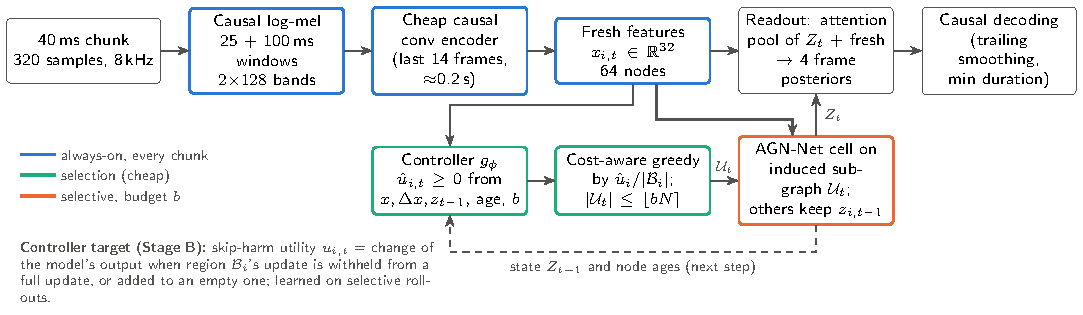
\includegraphics[width=\linewidth]{figures/overview.pdf}
\end{adjustwidth}
\caption{Overview of Event-Aware AGN-Net. Each 40\,ms chunk is processed by a causal two-resolution log-mel front end and a cheap convolutional encoder, giving fresh features $x_{i,t}$ for $N{=}64$ frequency-region nodes. A controller scores each seed region $\B_i$, and a cost-aware greedy picks an update set $\U_t$ whose size never exceeds $\lfloor bN\rceil$. The AGN-Net cell updates only the nodes in $\U_t$, on the subgraph induced by $\U_t$; all other nodes keep their state. The readout combines the pooled graph state with the fresh features. The controller is trained to predict the \emph{skip-harm utility}, i.e., how much the output changes when a region's update is withheld.}
\label{fig:overview}
\end{figure}

\subsection{Problem Formulation}
Audio arrives in 40\,ms chunks. After chunk $t$, the model must output class posteriors for the four 10\,ms frames in that chunk, using only audio received so far. There are $C{=}8$ classes: background plus the seven SPRSound event types (Normal, Rhonchi, Wheeze, Stridor, Coarse Crackle, Fine Crackle, Wheeze+Crackle). Events are decoded from the frame posteriors. The model keeps a state $z_{i,t}$ for each of $N$ graph nodes. A budget $b\in(0,1]$ limits how many node states may be recomputed per chunk. The goal is to choose, at each step, the update set $\U_t$ with $|\U_t|\le\lfloor bN\rceil$ that keeps the output as close as possible to the output of updating every node ($\lfloor\cdot\rceil$ denotes rounding to the nearest integer).

\subsection{Always-On Encoder}
Audio is processed at its native 8\,kHz. For each 10\,ms frame we compute two log-mel spectra (128 bands, 50--4000\,Hz) with 25\,ms and 100\,ms Hann windows that end at the current frame, so no future samples are used. Features are standardized with fixed statistics from the training set. A causal $5{\times}3$ convolution (2$\to$16 channels) runs at the frame rate, the four frames of a chunk are averaged, and a second causal $5{\times}3$ convolution (16$\to$32 channels, frequency stride 2) runs at the chunk rate, followed by LayerNorm. This gives a 32-dimensional feature $x_{i,t}$ for each of the 64 frequency regions. The encoder only sees the last 14 frames (about 0.2\,s), so longer temporal context must come from the graph state.

\subsection{Persistent Acoustic Graph}
\DIFaddbegin \label{sec:graph}
\DIFaddend Each node $i$ is anchored to a fixed pair of adjacent mel channels at both resolutions, so its identity is stable over time while its features change. Edges connect nodes at frequency distance 1 and 2. \DIFaddbegin \DIFadd{This chain is the simplest topology, and it cannot pass evidence between distant harmonics in one step. Wheezes and stridor are (quasi-)harmonic, with energy at integer multiples of a fundamental frequency, so we also build a }\emph{\DIFadd{harmonic graph}} \DIFadd{that additionally links each node to the nodes nearest to twice and three times its centre frequency (relative mismatch below 6\%). This adds 82 edges, with at most 8 neighbours per node. Selection, budgets and training are unchanged; only the regions $\B_i$ become larger. }\DIFaddend Each node keeps a 96-dimensional state. For nodes in the update set $\U_t$, the AGN-Net cell computes
\DIFdelbegin \begin{align*}
\DIFdel{h^{(0)}_i }&\DIFdel{= \mathrm{GELU}\big(W_{\mathrm{in}}[x_{i,t};z_{i,t-1}] + e_i\big),}\\
\DIFdel{h^{(\ell)}_i }&\DIFdel{= \mathrm{ELU}\Big(\sum_{j\in\mathcal{N}_{\U}(i)}\alpha^{(\ell)}_{ij}W^{(\ell)}h^{(\ell-1)}_j+\beta_\ell h^{(\ell-1)}_i\Big),}\\
\DIFdel{f_i }&\DIFdel{= \mathrm{LN}\Big(\textstyle\sum_{\ell=0}^{2}\mathrm{softmax}(w)_\ell\,h^{(\ell)}_i\Big),}\\
\DIFdel{c_i }&\DIFdel{= \tanh(\mathrm{MLP}(f_i)),}\\
\DIFdel{\lambda_i }&\DIFdel{= \sigma\big(w_g^\top[f_i;z_{i,t-1}]+b_g\big),}\\
\DIFdel{z_{i,t} }&\DIFdel{= (1-\lambda_i)\,z_{i,t-1}+\lambda_i\,c_i,
}\end{align*}%DIFAUXCMD
\DIFdelend \DIFaddbegin \begin{align}
\DIFadd{h^{(0)}_i }&\DIFadd{= \mathrm{GELU}\big(W_{\mathrm{in}}[x_{i,t};z_{i,t-1}] + e_i\big),\label{eq:cell-first}}\\
\DIFadd{h^{(\ell)}_i }&\DIFadd{= \mathrm{ELU}\Big(\sum_{j\in\mathcal{N}_{\U}(i)}\alpha^{(\ell)}_{ij}W^{(\ell)}h^{(\ell-1)}_j+\beta_\ell h^{(\ell-1)}_i\Big),}\\
\DIFadd{f_i }&\DIFadd{= \mathrm{LN}\Big(\textstyle\sum_{\ell=0}^{2}\mathrm{softmax}(w)_\ell\,h^{(\ell)}_i\Big),}\\
\DIFadd{c_i }&\DIFadd{= \tanh(\mathrm{MLP}(f_i)),}\\
\DIFadd{\lambda_i }&\DIFadd{= \sigma\big(w_g^\top[f_i;z_{i,t-1}]+b_g\big),}\\
\DIFadd{z_{i,t} }&\DIFadd{= (1-\lambda_i)\,z_{i,t-1}+\lambda_i\,c_i,\label{eq:cell-update}
}\end{align}\DIFaddend 
for layers $\ell=1,2$. Nodes outside $\U_t$ keep their state, $z_{i,t}=z_{i,t-1}$. Here GELU and ELU are the Gaussian-error and exponential linear units, LN is layer normalization, MLP is a multilayer perceptron, $e_i$ is a learned node embedding, $\alpha^{(\ell)}_{ij}$ are graph-attention weights~\cite{velickovic2018graph} computed only over neighbours inside $\U_t$ (AGN-Net's induced-subgraph update~\cite{islam2026agnnet}), $\beta_\ell$ are learned residual weights, and $w$ fuses the layers. AGN-Net's temporal-momentum update is kept, with its global momentum replaced by a per-node gate $\lambda_i$. When $\U_t$ contains all nodes, we call the model the \emph{full-update} model. \DIFaddbegin \DIFadd{For the plain graph-GRU cell used in Section~\ref{sec:generality}, $z_{i,t}=\mathrm{GRU}\big(\mathrm{GELU}(W[x_{i,t};\bar z_{\mathcal{N}(i),t-1}]+e_i),\,z_{i,t-1}\big)$ with $\bar z_{\mathcal{N}(i)}$ the mean of the neighbour states; a selective update applies this only to $i\in\U_t$ and reads the (possibly stale) states of all neighbours, so for this cell the boundary defect of Proposition~\ref{prop:bound} is zero.

}\DIFaddend 

The readout pools the node states with attention, $g_t=\sum_i\mathrm{softmax}_i(w_s^\top z_{i,t})\,z_{i,t}$, concatenates the mean and maximum of the fresh features over nodes, and maps the result through a two-layer MLP to four frame posteriors. The fresh-feature input lets the readout react to the current chunk even when few states were updated. The full model has about 108,000 parameters.

\subsection{Budgeted Region Selection}
\label{sec:selection}
Selecting a seed node $i$ updates its region $\B_i=\{i\}\cup\mathcal{N}(i)$ of 3--5 nodes \DIFaddbegin \DIFadd{(up to 9 on the harmonic graph)}\DIFaddend , so the actual update set is the union of the selected regions. We therefore count the budget in updated nodes, $|\U_t|\le\lfloor bN\rceil$, not in seeds. Each policy gives every region a non-negative score $s_{i,t}$ (a region total). A greedy rule visits the regions in decreasing order of the per-node score $s_{i,t}/|\B_i|$, and adds a region if it brings at least one new node and still fits the budget. This is a heuristic for a budgeted coverage problem~\cite{khuller1999budgeted}. We use the per-node score, rather than the usual score per newly covered node, because the latter makes regions overlapping an already chosen region look almost free, and the update set then grows as one contiguous block regardless of score.

To avoid states becoming arbitrarily stale, nodes whose state is at least \DIFdelbegin \DIFdel{50 steps (2\,s) }\DIFdelend \DIFaddbegin \DIFadd{$A$ steps }\DIFaddend old are refreshed first. These refreshes count against the same budget. As a result, every policy performs exactly the same number of node updates per step. \DIFaddbegin \DIFadd{Refreshing all $N$ nodes once every $A$ steps costs at most $N/A$ updates per step, i.e., a share $1/(Ab)$ of the budget, so a fixed threshold weighs most on the smallest budgets. The main experiments use a fixed $A{=}50$ steps (2\,s). On long streams (Section~\ref{sec:long}) we also test a budget-adaptive threshold $A(b)=\lceil 12.5/b\rceil$ steps (100, 50 and 25 steps at 12.5\%, 25\% and 50\%), which caps the refresh share at 8\% of the budget.

}\DIFaddend 

\subsection{Skip-Harm Utility}
\label{sec:utility}
The controller should prefer regions whose update matters for the output. We measure this directly with one-step counterfactuals. Let $p(Z)$ be the readout's frame posteriors for state $Z$, and $p^{\mathrm{full}}$ and $p^{\mathrm{none}}$ the posteriors if all or no nodes are updated at this step. For region $i$, let $p^{\mathrm{hold}(i)}$ be the posteriors when every node except $\B_i$ is updated, and $p^{\mathrm{only}(i)}$ when only $\B_i$ is updated. With $D$ the Kullback--Leibler (KL) divergence averaged over the four frames, we define
\begin{align}
\Delta^{\mathrm{hold}}_{i,t} &= D\big(p^{\mathrm{full}}\,\|\,p^{\mathrm{hold}(i)}\big),\nonumber\\
\Delta^{\mathrm{add}}_{i,t} &= \big(D(p^{\mathrm{full}}\|p^{\mathrm{none}})-D(p^{\mathrm{full}}\|p^{\mathrm{only}(i)})\big)_+,\nonumber\\
L^{\mathrm{hold}}_{i,t} &= \big(\mathrm{CE}(y,p^{\mathrm{hold}(i)})-\mathrm{CE}(y,p^{\mathrm{full}})\big)_+,\nonumber\\
L^{\mathrm{add}}_{i,t} &= \big(\mathrm{CE}(y,p^{\mathrm{none}})-\mathrm{CE}(y,p^{\mathrm{only}(i)})\big)_+,\nonumber\\
u_{i,t} &= \tfrac12\big(\Delta^{\mathrm{hold}}_{i,t}+\Delta^{\mathrm{add}}_{i,t}\big)+\tfrac{\mu}{2}\big(L^{\mathrm{hold}}_{i,t}+L^{\mathrm{add}}_{i,t}\big),
\label{eq:utility}
\end{align}
where $\mathrm{CE}$ is the frame cross-entropy on labelled frames and $\mu{=}1$. The $\Delta$ terms measure how much the prediction depends on region $i$ when it is removed from a full update and when it is added to an empty one. This two-point estimate is similar in spirit to a Shapley value~\cite{lundberg2017unified}. The $L$ terms add the increase in supervised loss. Computing the targets is cheap: one cell evaluation plus 128 readout evaluations per step for all 64 regions, run on the graphics processing unit (GPU) without gradients. For speed, the intervened regions reuse the state computed with their full neighbourhood.

\DIFaddbegin 

\DIFaddend The targets are one-step proxies\DIFdelbegin \DIFdel{and do not model the later effects of a skip. }\DIFdelend \DIFaddbegin \DIFadd{. A skipped state stays stale, so a skip can also change later outputs, and repeated skips of the same region compound. Exact multi-step targets would require rolling out every region's counterfactual over the horizon, which multiplies the cost of target generation by the horizon length and makes the target depend on future selections. We therefore keep the one-step target and test directly, in Section~\ref{sec:multistep}, how well it ranks regions by their measured harm over horizons of up to 1\,s and under repeated skips.

}\DIFaddend 

\paragraph*{Controller}
The controller uses only information available at inference time: $r_{i,t}=[x_{i,t};\,x_{i,t}-x_{i,t-1};\,z_{i,t-1};\,a_{i,t};\,b]$, where $a_{i,t}$ is the (log-scaled) age of node $i$'s state. A shared per-node layer (24 units) is followed by a 5-tap convolution over neighbouring nodes and a softplus output $\hat u_{i,t}\ge0$, for about 6800 parameters in total. It is trained with a Huber loss between $\log(1+\hat u_{i,t})$ and $\log(1+u_{i,t}/\kappa)$, where $\kappa$ is a fixed target scale ($\kappa{=}0.01$; $0.1$ for the change head below). With the same architecture, inputs and training data we also train three alternative heads: a \emph{change} head that predicts the representation change $\|z^{\mathrm{full}}_{j,t}-z_{j,t-1}\|$ averaged over the region (AGN-Net's objective), a \emph{hold-only} head ($\Delta^{\mathrm{hold}}+\mu L^{\mathrm{hold}}$), and a \emph{label-free} head ($\mu{=}0$).

\subsection{Training}
\label{sec:training}
Training has three stages. \emph{Stage A} trains the encoder, cell and readout with full updates for 40 epochs, using AdamW (peak learning rate $2{\times}10^{-3}$, one-cycle schedule), batches of 32 random 8\,s crops, class-weighted frame cross-entropy, random gain, and frequency masking~\cite{park2019specaugment}. \emph{Stage B} freezes the model and trains the controller heads for 6 epochs on \emph{selective rollouts}. Each batch runs either random selection or one of the learned heads under a random budget, so the controllers see the stale states they will meet at inference time~\cite{ross2011reduction}. \emph{Stage C} fine-tunes the model for 8 epochs under a random policy and budget per batch, with a distillation loss~\cite{hinton2015distilling} towards the stage-A full-update model. The controllers are then refreshed for 2 epochs \DIFaddbegin \DIFadd{on the fine-tuned model (stage B$'$)}\DIFaddend . Because one fine-tuned model serves all policies, every policy is evaluated on the same weights. Gradient clipping and a guard that skips non-finite updates keep training stable.

\subsection{Error Analysis}
\label{sec:theory}
Selective updating differs from full updating in two ways: nodes outside $\U_t$ keep stale states (\emph{skip defect}), and nodes inside $\U_t$ miss messages from neighbours outside it (\emph{boundary defect}). AGN-Net~\cite{islam2026agnnet} bounded the first; we add the second. Let \DIFdelbegin \DIFdel{both models share weights and inputs, start from $Z_0=0$, }\DIFdelend \DIFaddbegin \DIFadd{$V=\{1,\dots,N\}$ and equip the state space with the norm $\|Z\|_{\infty,2}=\max_{i\in V}\|z_i\|_2$. For the current input $x_t$, }\DIFaddend let \DIFdelbegin \DIFdel{$\Phi$ be the full-update transition, and let $e_t=\max_i\|z^{\mathrm{full}}_{i,t}-z^{\mathrm{sel}}_{i,t}\|_2$. }\DIFdelend \DIFaddbegin \DIFadd{$\Phi_t(Z)=\Phi(Z,x_t)$ denote the full-graph transition, i.e., Equations~(\ref{eq:cell-first})--(\ref{eq:cell-update}) applied to every node on the full graph. For $U\subseteq V$, let $\Phi_t^{U}$ denote the selective transition, which applies Equations~(\ref{eq:cell-first})--(\ref{eq:cell-update}) on the subgraph induced by $U$ to the nodes in $U$ and leaves the other states unchanged, $[\Phi_t^{U}(Z)]_i=z_i$ for $i\notin U$. Both models share weights and inputs and follow
}\[
\DIFadd{Z^{\mathrm{full}}_t=\Phi_t(Z^{\mathrm{full}}_{t-1}),\qquad Z^{\mathrm{sel}}_t=\Phi_t^{\U_t}(Z^{\mathrm{sel}}_{t-1}),\qquad Z^{\mathrm{full}}_0=Z^{\mathrm{sel}}_0,
}\]
\DIFadd{and we write $e_t=\|Z^{\mathrm{full}}_t-Z^{\mathrm{sel}}_t\|_{\infty,2}$.

}\DIFaddend 

\begin{Proposition}
\label{prop:bound}
Assume \DIFdelbegin \DIFdel{$\Phi(\cdot,x_t)$ }\DIFdelend \DIFaddbegin \DIFadd{that, for each $t$, $\Phi_t$ }\DIFaddend is $\gamma_t$-Lipschitz in \DIFdelbegin \DIFdel{the norm $\max_i\|\cdot\|_2$. Let $\delta^{\mathrm{skip}}_t=\max_{i\notin\U_t}\lambda_i\|c_i-z^{\mathrm{sel}}_{i,t-1}\|_2$ and $\delta^{\mathrm{bnd}}_t=\max_{i\in\U_t}\|\Phi_i(Z^{\mathrm{sel}}_{t-1})-\Phi^{\U_t}_i(Z^{\mathrm{sel}}_{t-1})\|_2$}\DIFdelend \DIFaddbegin \DIFadd{$\|\cdot\|_{\infty,2}$ on a domain that contains the states of both trajectories, with $\gamma_t\ge0$. Define the skip and boundary defects}\DIFaddend , both evaluated at the selective \DIFdelbegin \DIFdel{state. Then $e_t\le\gamma_t e_{t-1}+\max\{\delta^{\mathrm{skip}}_t,\delta^{\mathrm{bnd}}_t\}$. If}\DIFdelend \DIFaddbegin \DIFadd{model's previous state,
}\[
\DIFadd{\delta^{\mathrm{skip}}_t=\max_{i\notin\U_t}\big\|\Phi_{t,i}(Z^{\mathrm{sel}}_{t-1})-z^{\mathrm{sel}}_{i,t-1}\big\|_2,\qquad
\delta^{\mathrm{bnd}}_t=\max_{i\in\U_t}\big\|\Phi_{t,i}(Z^{\mathrm{sel}}_{t-1})-\Phi^{\U_t}_{t,i}(Z^{\mathrm{sel}}_{t-1})\big\|_2,
}\]
\DIFadd{where a maximum over an empty node set is zero, and let $d_t=\max\{\delta^{\mathrm{skip}}_t,\delta^{\mathrm{bnd}}_t\}$. Then $e_t\le\gamma_t e_{t-1}+d_t$, and consequently
}\[
\DIFadd{e_t\le\sum_{s=1}^{t}\Big(\prod_{r=s+1}^{t}\gamma_r\Big)\,d_s ,
}\]
\DIFadd{where an empty product equals one. If, in addition, }\DIFaddend $\gamma_t\le\gamma<1$ and \DIFdelbegin \DIFdel{both defects are at most $\bar\delta$}\DIFdelend \DIFaddbegin \DIFadd{$d_t\le\bar\delta$ for all $t$}\DIFaddend , then $e_t\le\bar\delta(1-\gamma^t)/(1-\gamma)$.
\end{Proposition}
\begin{proof}
\DIFdelbegin \DIFdel{Write $Z^{\mathrm{full}}_t-Z^{\mathrm{sel}}_t=[\Phi(Z^{\mathrm{full}}_{t-1})-\Phi(Z^{\mathrm{sel}}_{t-1})]+[\Phi(Z^{\mathrm{sel}}_{t-1})-Z^{\mathrm{sel}}_t]$. The first term is at most }\DIFdelend \DIFaddbegin \DIFadd{Add and subtract $\Phi_t(Z^{\mathrm{sel}}_{t-1})$. By the triangle inequality,
}\[
\DIFadd{e_t\le\big\|\Phi_t(Z^{\mathrm{full}}_{t-1})-\Phi_t(Z^{\mathrm{sel}}_{t-1})\big\|_{\infty,2}+\big\|\Phi_t(Z^{\mathrm{sel}}_{t-1})-\Phi_t^{\U_t}(Z^{\mathrm{sel}}_{t-1})\big\|_{\infty,2}.
}\]
\DIFadd{The Lipschitz assumption bounds the first term by }\DIFaddend $\gamma_t e_{t-1}$. \DIFdelbegin \DIFdel{Row by row , the }\DIFdelend \DIFaddbegin \DIFadd{In the second term, skipped nodes keep their previous states, so the maximum row norm over $V\setminus\U_t$ is $\delta^{\mathrm{skip}}_t$, and the maximum row norm over $\U_t$ is $\delta^{\mathrm{bnd}}_t$. The two row sets are disjoint and cover $V$, so the }\DIFaddend second term equals \DIFdelbegin \DIFdel{the skip defect for nodes outside $\U_t$ and the boundary defect for nodes inside, so its norm is their maximum. Unrolling with }\DIFdelend \DIFaddbegin \DIFadd{$d_t$. Hence $e_t\le\gamma_t e_{t-1}+d_t$. Iterating gives $e_t\le(\prod_{r=1}^{t}\gamma_r)\,e_0+\sum_{s=1}^{t}(\prod_{r=s+1}^{t}\gamma_r)\,d_s$, and }\DIFaddend $e_0=0$\DIFdelbegin \DIFdel{gives the geometric bound }\DIFdelend \DIFaddbegin \DIFadd{. Under $\gamma_t\le\gamma<1$ and $d_t\le\bar\delta$, the sum is at most $\bar\delta\sum_{k=0}^{t-1}\gamma^k=\bar\delta(1-\gamma^t)/(1-\gamma)$}\DIFaddend .
\end{proof}

\DIFdelbegin \DIFdel{The bound shows that a smallupdate fraction alone guarantees nothing: the error depends on how large the skipped and boundary defects are . What matters for the prediction, however, }\DIFdelend \DIFaddbegin \DIFadd{For the gated AGN-Net cell, Equation~(\ref{eq:cell-update}) gives an equivalent form of the skip defect: $\Phi_{t,i}(Z^{\mathrm{sel}}_{t-1})-z^{\mathrm{sel}}_{i,t-1}=\lambda^{F}_{i,t}\,(c^{F}_{i,t}-z^{\mathrm{sel}}_{i,t-1})$, so $\delta^{\mathrm{skip}}_t=\max_{i\notin\U_t}\lambda^{F}_{i,t}\|c^{F}_{i,t}-z^{\mathrm{sel}}_{i,t-1}\|_2$, where the gate $\lambda^{F}_{i,t}\ge0$ and the candidate $c^{F}_{i,t}$ are computed on the }\emph{\DIFadd{full}} \DIFadd{graph from $Z^{\mathrm{sel}}_{t-1}$, a hypothetical update that the selective model does not perform. Defined through $\Phi_t$, the proposition applies unchanged to the graph-GRU cell, whose boundary defect }\DIFaddend is \DIFdelbegin \DIFdel{the error }\emph{\DIFdel{after the readout}}%DIFAUXCMD
\DIFdel{, which ignores state directions the readout }\DIFdelend \DIFaddbegin \DIFadd{zero (Section~\ref{sec:graph}). The argument is a standard perturbation analysis, in which a one-step Lipschitz bound is iterated into a geometric series, as for the hidden states of simple recurrent networks~\mbox{%DIFAUXCMD
\cite{mitarchuk2024length}}\hskip0pt%DIFAUXCMD
; the application-specific part is the decomposition into skipped-update and induced-subgraph defects.

}

\DIFadd{The result is a conditional error-propagation bound. It does not show that the learned transition contracts, that the controller makes either defect small, that a given budget guarantees a given error, or that the greedy selection minimises the bound. The gate alone does not imply contraction: for the scalar map $\Phi(z)=\tfrac12 z+\tfrac12\tanh(2z)$, which has a gate of $\tfrac12$ and a bounded candidate, $\Phi'(0)=\tfrac32>1$. The uniform condition $\gamma_t\le\gamma<1$ is therefore a substantive assumption, which nothing in training enforces. On the observed trajectories we can, however, measure the secant ratio
}\[
\DIFadd{\hat\gamma_t=\begin{cases}\big\|\Phi_t(Z^{\mathrm{full}}_{t-1})-\Phi_t(Z^{\mathrm{sel}}_{t-1})\big\|_{\infty,2}\,/\,e_{t-1}, & e_{t-1}>0,\\ 0, & e_{t-1}=0,\end{cases}
}\]
\DIFadd{which satisfies the recurrence with $\gamma_t$ replaced by $\hat\gamma_t$ (when $e_{t-1}=0$ the numerator is zero as well, because transition and input are shared). The recurrence with $\hat\gamma_t$ is an a~posteriori bound for these trajectories, valid also on steps with $\hat\gamma_t>1$; it says nothing about other pairs of states. We measure $\hat\gamma_t$ in Section~\ref{sec:lip}.

}

\DIFadd{The bound concerns the state, whereas the prediction depends on the frame posteriors. Hold the fresh features fixed, as both models share them, and suppose the readout maps states to frame logits with Lipschitz constant $L_R$ (state norm $\|\cdot\|_{\infty,2}$, logits in the max norm). Since log-sum-exp is 1-Lipschitz in the max norm, $\|\log p-\log q\|_\infty\le2\|a-b\|_\infty$ for $p=\mathrm{softmax}(a)$ and $q=\mathrm{softmax}(b)$, and therefore, for every frame and for the frame average,
}\begin{equation}
\DIFadd{\mathrm{KL}\big(p^{\mathrm{full}}_t\,\|\,p^{\mathrm{sel}}_t\big)\;\le\;2L_R\,e_t .
\label{eq:readout}
}\end{equation}
\DIFadd{A small KL divergence alone does not guarantee the same predicted class: the logits $(\varepsilon,0)$ and $(0,\varepsilon)$ have different arg-max labels for every $\varepsilon>0$, while their KL divergence tends to zero. A sufficient condition for keeping a frame's arg-max label is a full-model logit margin $m_t>2L_Re_t$, where $m_t$ is the difference between the largest and second-largest full-model logits; preserving decoded events further depends on the temporal decoding rules. Eq.~(\ref{eq:readout}) thus links the state bound to the KL-based skip-harm objective, but only as an upper bound: the readout ignores state directions it }\DIFaddend does not use\DIFaddbegin \DIFadd{, so a large state error can leave the output unchanged}\DIFaddend . The skip-harm utility measures \DIFdelbegin \DIFdel{exactly this }\DIFdelend \DIFaddbegin \DIFadd{the }\DIFaddend output-level effect of a skip \DIFdelbegin \DIFdel{, which motivates }\DIFdelend \DIFaddbegin \DIFadd{directly, which is why we use }\DIFaddend it as the training target \DIFaddbegin \DIFadd{rather than a state-level quantity. Section~\ref{sec:lip} quantifies how loose the link is}\DIFaddend .
\DIFdelbegin \DIFdel{The bound is conditional: the Lipschitz assumption isnot guaranteed for the trained network, and the bound says nothing directly about event recall.
}\DIFdelend 

\section{Experiments}
\label{sec:experiments}

We design the experiments to answer five questions. \textbf{RQ1:} Which updates can be skipped, i.e., does the skip-harm controller preserve the full model's detections better than other selection policies\DIFaddbegin \DIFadd{, including a gate trained end to end on the task loss, }\DIFaddend at the same budget? \textbf{RQ2:} Why does it work\DIFaddbegin \DIFadd{, and is the one-step target sufficient}\DIFaddend ? \textbf{RQ3:} Does it carry over to \DIFdelbegin \DIFdel{a different graph cell}\DIFdelend \DIFaddbegin \DIFadd{other cells, another graph topology and another dataset}\DIFaddend ? \textbf{RQ4:} Which design choices matter\DIFaddbegin \DIFadd{, including the refresh rule on long streams}\DIFaddend ? \textbf{RQ5:} Does selective updating reduce end-to-end latency\DIFaddbegin \DIFadd{, and how does the controller's overhead scale}\DIFaddend ? We also compare the full-update backbones. \DIFaddbegin \DIFadd{Throughout, the primary question is how well selective inference }\emph{\DIFadd{preserves}} \DIFadd{what the same model detects with full updates; accuracy against the annotations is reported as a secondary check, because absolute scores on this benchmark are dominated by an annotation-style shift (Section~\ref{sec:data}).

}\DIFaddend 

\subsection{Dataset}
\label{sec:data}
We use SPRSound~\cite{zhang2022sprsound} with the data splits of the BioCAS 2024 event-detection challenge~\cite{zhang2024meta}: the official detection training and validation recordings for development, and the 2024 test set (1704 recordings) for testing. We use the later 2025 release (1309 recordings)~\cite{sprsound2025repo} only as an additional test set. All audio is 8\,kHz. An audit of the official split showed that the validation set shares 261 of its 266 patients with the training set. We therefore pooled the two, removed duplicates, and held out 15\% of the patients as a patient-disjoint validation set. The test sets are effectively patient-disjoint from training. Table~\ref{tab:data} summarizes the data.

\DIFaddbegin \DIFadd{To test whether the findings carry over to adult lung sounds and another recording setup, we also use HF\_Lung\_V1~\mbox{%DIFAUXCMD
\cite{hsu2021benchmarking} }\hskip0pt%DIFAUXCMD
(CC BY 4.0): 9765 fifteen-second recordings from 279 adults, made with a Littmann 3200 stethoscope or a multichannel acoustic device, with onset/offset labels for inhalation (I), exhalation (E), discontinuous adventitious sounds (D, crackles), and continuous adventitious sounds (wheeze, stridor, rhonchi). The audio is 4\,kHz; we resample it to 8\,kHz so that the front end is unchanged. Phase and adventitious labels overlap, while our detector predicts one class per frame, so each frame takes the highest-priority label present (wheeze, stridor, rhonchi, D, E, I, background, in that order), and reference events are the maximal runs of the resolved labels. We keep the official train/test split and hold out 15\% of the training subjects for validation. Recordings are not labelled by patient, so subjects are approximated by recording device and date, as the dataset documentation recommends; this gives the 171 pseudo-subjects of Table~\ref{tab:data} for the 279 patients, and the split is disjoint in these groups. HF\_Lung has 3.1 times as much training audio as SPRSound, so we shorten the schedules (Section~\ref{sec:impl}) to keep the number of gradient steps similar.

}

\DIFaddend \begin{table}[H]
\caption{Data splits. ``Adv.'' counts adventitious (abnormal) events. \DIFaddbeginFL \DIFaddFL{HF\_Lung subjects are approximated by recording device and date, as the dataset documentation recommends; HF\_Lung events are counted after overlapping labels are resolved (Section~\ref{sec:data}).}\DIFaddendFL }
\label{tab:data}
\centering
\setlength{\tabcolsep}{3.5pt}
\DIFdelbeginFL %DIFDELCMD < \begin{tabular}{lrrrrr}
%DIFDELCMD < \toprule
%DIFDELCMD < \textbf{Split} & \textbf{Recordings} & \textbf{Patients} & \textbf{Hours} & \textbf{Events} & \textbf{Adv.} \\
%DIFDELCMD < \midrule
%DIFDELCMD < Train & 2698 & 320 & 8.5 & 9952 & 2206 \\
%DIFDELCMD < Validation & 625 & 56 & 1.9 & 2260 & 661 \\
%DIFDELCMD < Test 2024 & 1704 & 324 & 5.9 & 7659 & 407 \\
%DIFDELCMD < Test 2025 & 1309 & 162 & 3.9 & 4706 & 2531 \\
%DIFDELCMD < \bottomrule
%DIFDELCMD < \end{tabular}
%DIFDELCMD < %%%
\DIFdelendFL \DIFaddbeginFL \begin{tabular}{lrrrrr}
\toprule
\textbf{Split} & \textbf{Recordings} & \textbf{Patients} & \textbf{Hours} & \textbf{Events} & \textbf{Adv.} \\
\midrule
\multicolumn{6}{l}{\textit{SPRSound (paediatric)}} \\
Train & 2698 & 320 & 8.5 & 9952 & 2206 \\
Validation & 625 & 56 & 1.9 & 2260 & 661 \\
Test 2024 & 1704 & 324 & 5.9 & 7659 & 407 \\
Test 2025 & 1309 & 162 & 3.9 & 4706 & 2531 \\
\midrule
\multicolumn{6}{l}{\textit{HF\_Lung\_V1 (adult)}} \\
Train & 6403 & 110 & 26.7 & 45,398 & 21,095 \\
Validation & 1406 & 20 & 5.9 & 7865 & 3955 \\
Test & 1956 & 41 & 8.2 & 11,541 & 4224 \\
\bottomrule
\end{tabular}
\DIFaddendFL \end{table}

The test sets also follow a different annotation style from the training data (Table~\ref{tab:shift}). In training, events cover 45\% of a recording and are separated by gaps of about 0.4\,s. In the 2024 test set, events cover 76\% of the recording and almost touch each other. The 2025 set has the same style and a much higher share of adventitious events. Detectors trained on the training style are therefore penalized by strict onset/offset matching on the test sets, which keeps absolute event scores low for every model.

\begin{table}[H]
\caption{Annotation statistics differ between releases (durations in seconds; median [interquartile range]).}
\label{tab:shift}
\centering
\setlength{\tabcolsep}{4pt}
\resizebox{\columnwidth}{!}{%
\begin{tabular}{lccc}
\toprule
\textbf{Statistic} & \textbf{Train} & \textbf{Test 2024} & \textbf{Test 2025} \\
\midrule
Event coverage of recording & 45\% & 76\% & 68\% \\
Event duration & 1.30 [0.93, 1.76] & 2.06 [1.64, 2.51] & 1.92 [1.62, 2.31] \\
Gap between events & 0.39 [0.09, 1.01] & 0.04 [0.03, 0.06] & 0.08 [0.06, 0.12] \\
Adventitious share of events & 22\% & 5\% & 54\% \\
\bottomrule
\end{tabular}}
\end{table}

\subsection{Evaluation Metrics}
\label{sec:metrics}
\paragraph*{Event preservation} Our main metric asks whether selective updating keeps what the same model detects with full updates. We decode events from both the full-update and the selective posteriors, and compute the event-based F-score of the selective events against the full-update events ($F_{\mathrm{pres}}$). We also report $R^{\mathrm{adv}}_{\mathrm{pres}}$, the fraction of the full model's adventitious detections that the selective model also produces. These metrics do not depend on the annotation style. They measure agreement with the model's own detections, not correctness, so we always report them together with metrics against the annotations.

\paragraph*{Detection against the annotations} We report the event-based F-score ($F$) used by the challenge~\cite{zhang2024meta}, computed as in~\cite{mesaros2016metrics}, with DCASE-style collars~\cite{turpault2019sound}: 200\,ms at the onset, and the larger of 200\,ms and 20\% of the event duration at the offset. The official evaluator is not public, so these settings are ours. We also report the 1\,s segment-based F-score for adventitious classes (seg-adv-$F$), which is less sensitive to the annotation style, and the SPRSound harmonic score (HS) for classifying annotated segments~\cite{zhang2022grand}. \DIFaddbegin \DIFadd{To separate boundary conventions from detection errors, we additionally compute boundary-tolerant variants: event $F$ with 0.5\,s and 1\,s collars, onset-only matching, ``any overlap'' matching (same class, overlapping in time), and segment-based $F$ over all classes with 1\,s and 2\,s segments. Each variant is computed both against the annotations and, for preservation, against the full model's own events.

}\DIFaddend 

\paragraph*{Decoding} Posteriors are smoothed with a trailing moving average, so no future frames are used, and runs shorter than a minimum length are dropped. Both parameters are chosen on the validation set.

\subsection{Compared Methods}
\label{sec:policies}
\paragraph*{Selection policies} All policies run on the same trained weights, with the same greedy rule, budget accounting and refresh rule. We evaluate them at budgets of 12.5\%, 25\% and 50\% of nodes per step:
\emph{random}; \emph{periodic} (stalest regions first, i.e., round-robin); \emph{energy} (highest band-relative log-mel energy); \emph{acoustic change} (largest spectral change); \emph{change} (the learned head trained on representation change, i.e., AGN-Net's objective); two ablations of our target (\emph{hold-only} and \emph{label-free}); and our \emph{skip-harm} controller. As a reference, a \emph{hindsight oracle} computes the label-free utility by running the full update at every step. It is not available at inference time and is not budget-matched in computation. We also report the cheap path alone, with no graph updates.

\DIFaddbegin \paragraph*{\DIFadd{End-to-end gate}} \DIFadd{Skip RNN~\mbox{%DIFAUXCMD
\cite{campos2018skip} }\hskip0pt%DIFAUXCMD
and related gates are trained end to end through the task loss rather than on a surrogate target. As a baseline of this kind, we train a gate with the same architecture, inputs and parameter count as our controller, on the same stage-C weights, through the task loss of stage C (class-weighted cross-entropy plus distillation to the full-update model). Unlike Skip RNN, the backbone stays frozen while the gate is trained; moreover, stage C fine-tuned the backbone under a policy mixture that includes the utility heads but not this gate. The comparison therefore isolates the training signal of the selector and may favour our controller to an unknown degree. Its scores feed the same budget-exact greedy rule at training and at test time, so the budget is met exactly rather than on average and no budget penalty is needed. Gradients reach the gate through a straight-through relaxation~\mbox{%DIFAUXCMD
\cite{bengio2013estimating,jang2017categorical}}\hskip0pt%DIFAUXCMD
: in the forward pass the update set is the hard greedy selection on Gumbel-perturbed scores (Gumbel-noise scale annealed from 0.5 to 0.05); in the backward pass node $j$ has a soft inclusion $q_j=\sigma((\log s_j/|\B_j|-\theta)/\tau)$, where $\sigma$ is the logistic sigmoid, $\tau{=}1$ a fixed relaxation temperature and $\theta$ the $(1-b)$ quantile of the log scores, and the state update is $z_j\leftarrow m_j z^{\mathrm{cand}}_j+(1-m_j)z_j$ with $m_j=\mathbb{1}[j\in\U_t]+q_j-\mathrm{sg}(q_j)$, where $\mathrm{sg}(\cdot)$ is the stop-gradient operator. The candidate state is the selective update for selected nodes and the full update for the others, so unselected nodes also receive a task gradient. Back-propagation runs through the whole 8\,s crop. The gate is trained for 6 epochs with Adam (learning rate $2{\times}10^{-3}$), as long as stage B; we did not tune these settings, nor the temperatures.

}

\paragraph*{\DIFadd{Other cells and topology}} \DIFadd{To test generality, the same selection pipeline (stages A, B, C and B$'$ with unchanged hyperparameters) is applied to the plain graph-GRU cell and to the AGN-Net cell on the harmonic graph (Section~\ref{sec:method}).

}

\DIFaddend \paragraph*{Full-update backbones} To check whether the graph state itself is useful, we compare models that update every step and share our front end, encoder, readout and training recipe: attention \emph{pooling} without memory; a causal dilated \emph{temporal convolutional network} (TCN; receptive field about 5\,s); a \emph{GRU}; a plain \emph{graph GRU} (neighbour-mean aggregation with a shared GRU cell); a \emph{frequency-convolution} cell (our cell with attention replaced by a convolution over nodes); and our acoustic \emph{AGN-Net}. All use the same fixed recipe without per-model tuning.

\DIFaddbegin \subsection{\DIFadd{Additional Analyses}}
\label{sec:analyses}
\paragraph*{\DIFadd{Multi-step harm}} \DIFadd{On 150 validation recordings and the stage-C weights, we start from the full-update trajectory at every 15th step, hold region $\B_i$ for $k\in\{1,5,25\}$ consecutive steps while all other nodes are updated, then resume full updates, and sum the frame KL divergence to the full-update output over horizons $H\in\{1,5,25\}$ steps (up to 1\,s). We then measure, per step and across the 64 regions, the Spearman correlation between this multi-step harm and (i) the one-step utility, (ii) the trained controller's scores and (iii) the change head's scores.

}

\paragraph*{\DIFadd{Contraction and bound check}} \DIFadd{On the same recordings, we run the controller at each budget alongside the full-update model and record at every step the secant ratio $\hat\gamma_t$, both defects, the state error $e_t$, the readout ratio $\|\ell^{\mathrm{full}}_t-\ell^{\mathrm{sel}}_t\|_\infty/e_t$ between frame logits, and the frame KL divergence. This checks the assumptions and the conclusion of Proposition~\ref{prop:bound} on real trajectories.

}

\paragraph*{\DIFadd{Long streams}} \DIFadd{SPRSound recordings last 15\,s at most, too short for staleness to build up. We therefore concatenate the recordings of each test patient into one continuous stream of 60--120\,s, keeping the annotated events at their shifted times. This gives 141 streams (3.6\,h, mean 91\,s) from the 2024 test set and 66 (1.8\,h) from the 2025 release. We evaluate the controller with no refresh, fixed thresholds $A\in\{25,50,100,200\}$, and the adaptive $A(b)$, and also report the frame-level agreement with the full model (the share of frames whose most probable class matches) in the first 15\,s and after 30\,s of each stream.

}

\paragraph*{\DIFadd{Overhead scaling}} \DIFadd{To see how the controller's overhead changes when the cell is more expensive, we time the controller plus greedy selection and the graph update in the NumPy runtime (one pinned core, batch 1) for state sizes $d\in\{96,192,384,768\}$ and $L\in\{2,4\}$ message-passing layers. Weights are random, since arithmetic cost does not depend on their values; the controller's hidden size stays at 24.

}

\DIFaddend \subsection{Implementation Details}
\DIFaddbegin \label{sec:impl}
\DIFaddend All models are implemented in Python~3.11 with PyTorch~2.7.1 (CUDA~12.6) and trained on single GPUs (NVIDIA L4, L40S, A100 or H100). The event- and segment-based metrics use our own implementation, which is part of the released code. Every configuration is trained with three seeds. \DIFaddbegin \DIFadd{On HF\_Lung, stages A, B, C and B$'$ run for 15, 3, 3 and 1 epochs (40, 6, 8 and 2 on SPRSound), with all other settings unchanged. On HF\_Lung, three attempts with the AGN-Net cell (seed 2 twice, seed 3 once) diverged in stage A: around the peak of the learning-rate schedule, most batches began to give a non-finite loss, on two GPU types. The graph GRU never diverged. Because the same seed both diverged and trained normally on the same GPU type, the divergence stems from non-deterministic GPU arithmetic rather than from the seed. We therefore added a divergence rule to stage A (if more than 10\% of the batches of an epoch have a non-finite loss, the epoch's starting weights are restored and training continues with half the learning rate), which cannot affect a stable run, and repeated seed 2. This run had no non-finite batch, so the rule did not trigger. We report seeds 0, 1 and 2; the logs of the diverged attempts are released. This instability is specific to the AGN-Net cell and adds to the evidence that it is the less robust backbone (Section~\ref{sec:backbones}). }\DIFaddend Tables report the mean and standard deviation over seeds. For paired comparisons we use a patient-level bootstrap with 2000 resamples on counts pooled over seeds. Bootstrap differences are computed on these pooled counts\DIFdelbegin \DIFdel{and }\DIFdelend \DIFaddbegin \DIFadd{, which weight seeds and recordings by their event counts, and }\DIFaddend can therefore differ \DIFdelbegin \DIFdel{slightly }\DIFdelend from differences of the seed means reported in the tables \DIFdelbegin \DIFdel{. }\DIFdelend \DIFaddbegin \DIFadd{(e.g., 0.21 pooled vs.\ 0.18 from seed means for the end-to-end contrast at 25\%). }\DIFaddend Because this bootstrap treats the trained models as fixed, we also report whether a difference has the same sign in every seed. For non-inferiority of selective against full updating, we set a margin of $-0.01$ absolute event $F$ in advance. Selective updating is non-inferior if the lower bound of the 95\% interval of $F_{\mathrm{sel}}-F_{\mathrm{full}}$ is above this margin.

For latency we run batch-1 streaming on one pinned core of a central processing unit (CPU) server, with 60 test recordings per seed (about 20{,}000 chunks), and time each stage per chunk. We test two runtimes: a PyTorch implementation and a lightweight NumPy implementation of the same weights. Both perform true sparse updates (gather the selected nodes, compute on their subgraph, scatter back) and reproduce the batched model's outputs to within $3\times10^{-4}$. Configurations are interleaved per recording, and we report the median paired speedup over full updating on the same recording.

\DIFdelbegin \paragraph*{\DIFdel{Use of generative AI}} %DIFAUXCMD
\DIFdel{Generative AI }\DIFdelend \DIFaddbegin \subsection{\DIFadd{Use of Generative AI and Reproducibility}}
\label{sec:genai}
\DIFadd{An AI assistant }\DIFaddend (Claude Opus~5.5, Anthropic) was used \DIFaddbegin \DIFadd{extensively }\DIFaddend in this study\DIFdelbegin \DIFdel{to help write the experiment and analysis code, run }\DIFdelend \DIFaddbegin \DIFadd{, under the author's direction. Table~\ref{tab:genai} states which stages it performed. The research question and the central idea, training the update controller on the counterfactual consequence of skipping rather than on representation change, were the author's. The assistant proposed the detailed experimental protocol, wrote the code, ran }\DIFaddend the experiments on the \DIFdelbegin \DIFdel{computing cluster, analyse the results and draft }\DIFdelend \DIFaddbegin \DIFadd{university computing cluster under the author's account (every login required the author's two-factor approval), wrote the analysis scripts, drafted Proposition~\ref{prop:bound} and its proof, drafted the interpretation of the results and drafted }\DIFaddend the manuscript text. The author \DIFdelbegin \DIFdel{reviewed and verified all code}\DIFdelend \DIFaddbegin \DIFadd{set the research direction, made or approved every design and reporting decision, reviewed the code, results and text, and takes full responsibility for the content.

}

\DIFadd{Two measures make the results independent of the AI tool. First, every result value in the paper (all tables and figures and the results quoted in the text) is written into the manuscript from the result files by a script (}\texttt{\DIFadd{analyze.py}}\DIFaddend , \DIFdelbegin \DIFdel{results and text (see Acknowledgments). }\DIFdelend \DIFaddbegin \texttt{\DIFadd{analyze\_rev.py}}\DIFadd{, }\texttt{\DIFadd{render.py}}\DIFadd{), so a table cannot disagree with the logs; only dataset facts and a few rounded summary comparisons are typed in the text. Second, the complete code, configurations, job lists, training logs, per-recording results, trained weights and data splits are public at }\url{https://github.com/redwanUGA/event-aware-agn-net} \DIFadd{(release }\texttt{\DIFadd{v1.1-revision1}}\DIFadd{). Every table and figure can be regenerated from these files with the commands in the repository's README, without any AI tool; retraining needs only the public datasets and one GPU.

}\DIFaddend 

\DIFaddbegin \begin{table}[H]
\caption{\DIFaddFL{Division of work between the author and the AI assistant.}\label{tab:genai}}
\centering
\footnotesize
\begin{tabular}{p{0.34\textwidth}p{0.6\textwidth}}
\toprule
\textbf{Stage} & \textbf{Who} \\
\midrule
Research question, central idea & Author \\
Experimental design and protocol & Assistant proposed; author reviewed and approved \\
Code (models, training, metrics, runtimes) & Assistant wrote; author reviewed; released in full \\
Running experiments on the cluster & Assistant prepared and submitted the jobs; author approved every login \\
Interpretation of results and conclusions & Assistant drafted; author reviewed and decided \\
Literature search and citations & Assistant drafted; author reviewed \\
Statistical analysis, tables, figures & Assistant wrote the scripts; numbers are filled in automatically from logged results \\
Proposition~\ref{prop:bound} and its proof & Assistant drafted; author reviewed \\
Manuscript text and responses to reviewers & Assistant drafted; author revised and approved \\
\bottomrule
\end{tabular}
\end{table}


\DIFaddend \section{Results and Discussion}
\label{sec:results}

\policytable{tables/policy_C.tex}{Selection policies with the same number of node updates, all on the same weights. $F_{\mathrm{pres}}$: event preservation against the full-update model's own detections. $R^{\mathrm{adv}}_{\mathrm{pres}}$: share of the full model's adventitious detections that are preserved. $F$ and seg-adv-$F$: scores against the annotations. Bold: best policy per column and budget, excluding the hindsight oracle and the w/o-refresh ablation. $^\dagger$Hindsight oracle (runs the full update every step; not deployable). Mean$\pm$sd over three seeds.}{tab:policy}

\begin{figure}[H]
\begin{adjustwidth}{-\extralength}{0cm}
\centering
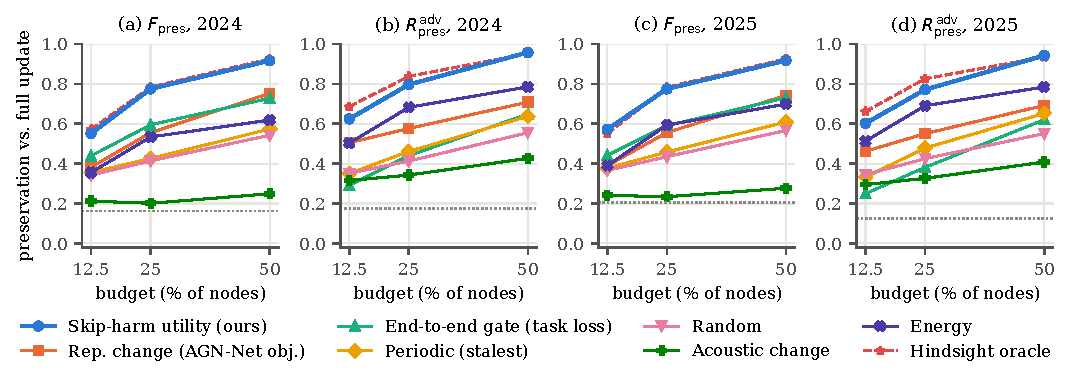
\includegraphics[width=\linewidth]{figures/budget_C.pdf}
\end{adjustwidth}
\caption{Preservation versus update budget (mean over seeds): (a) event preservation $F_{\mathrm{pres}}$, 2024 test set; (b) adventitious preservation $R^{\mathrm{adv}}_{\mathrm{pres}}$, 2024; (c) $F_{\mathrm{pres}}$, 2025 release; (d) $R^{\mathrm{adv}}_{\mathrm{pres}}$, 2025. The dotted line is the cheap path with no graph updates. Our skip-harm controller (blue) is above every non-utility baseline at every budget and close to the hindsight oracle (dashed). The hold-only variant, omitted here, lies close to ours; the label-free variant lies between ours and the change objective at 12.5\% and 25\% (Table~\ref{tab:policy}).}
\label{fig:budget}
\end{figure}

\subsection{Which Updates Can Be Skipped? (RQ1)}
Table~\ref{tab:policy} and Figure~\ref{fig:budget} compare the selection policies. Skipping matters: with no graph updates at all, event preservation drops to $F_{\mathrm{pres}}=0.163$, so the persistent state carries much of the information.

The skip-harm controller is the best deployable policy. With 25\% of the updates on the 2024 test set, it preserves the full model's events with $F_{\mathrm{pres}}=0.775$. AGN-Net's change objective reaches 0.555, energy 0.534, periodic refresh 0.425 and random selection 0.414. Our controller is close to the hindsight oracle (0.784). The gain is positive in every seed, by 0.14--0.60 over random and 0.11--0.41 over the change objective. The patient-level bootstrap gives 0.311 [0.304, 0.319] and 0.197 [0.189, 0.204], respectively ($p<0.001$). The same ordering holds at 12.5\% (0.552 vs.\ 0.382 and 0.342) and at 50\% (0.917 vs.\ 0.752 and 0.542). It also holds on the 2025 release (0.775 vs.\ 0.556 and 0.435 at 25\%) and for adventitious detections ($R^{\mathrm{adv}}_{\mathrm{pres}}=0.797$ vs.\ 0.576 and 0.413). Note that these are the model's own adventitious detections, few of which match an annotated adventitious event under the shifted annotation style.

\DIFaddbegin \paragraph*{\DIFadd{Comparison with end-to-end training}} \DIFadd{The gate trained end to end on the task loss is a competitive baseline, but it does not reach the two-stage controller. At 25\%, it preserves $F_{\mathrm{pres}}=0.595$ against 0.775 for our controller (bootstrap difference 0.212 }[\DIFadd{0.202, 0.222}]\DIFadd{), and our controller is better in every seed at every budget, by 0.07--0.35 at 25\%. On average the end-to-end gate is only slightly better than the change objective (0.555), and not in every seed. For the graph-GRU cell its results also vary strongly between seeds (Section~\ref{sec:gg}). Section~\ref{sec:why-two-stage} analyses why.

}

\DIFaddend \paragraph*{Accuracy against the annotations}
Better preservation \DIFaddbegin \DIFadd{than the heuristic baselines }\DIFaddend also gives better detection\DIFdelbegin \DIFdel{. }\DIFdelend \DIFaddbegin \DIFadd{, with one exception. The end-to-end gate, which preserves far fewer of the full model's events, scores slightly higher than our controller against the annotations at 25\% on the 2024 set (event $F$ 0.098; difference to ours }\ensuremath{-}\DIFadd{0.0056 }[\ensuremath{-}\DIFadd{0.0090, }\ensuremath{-}\DIFadd{0.0023}]\DIFadd{) and at 12.5\% on the 2025 release (}\ensuremath{-}\DIFadd{0.0032 }[\ensuremath{-}\DIFadd{0.0061, }\ensuremath{-}\DIFadd{0.0003}]\DIFadd{), whereas at 25\% on the 2025 release the two do not differ (0.0002 }[\ensuremath{-}\DIFadd{0.0026, 0.0034}]\DIFadd{) and at 50\% our controller is higher (0.0072 }[\DIFadd{0.0044, 0.0099}]\DIFadd{). Training directly on the task loss can thus trade fidelity to the full model for agreement with the shifted annotations. }\DIFaddend At 25\%, event $F$ against the annotations is 0.090 for our controller and 0.092 with full updates. Random and periodic selection change it by \ensuremath{-}0.046 and \ensuremath{-}0.044 (bootstrap estimates on pooled counts). For our controller the difference to full updating is \ensuremath{-}0.0026 [\ensuremath{-}0.0049, \ensuremath{-}0.0001]. Its lower bound is above the $-0.01$ margin, so selective inference with a quarter of the updates is non-inferior to full updating. The same holds on the 2025 release (\ensuremath{-}0.0002 [\ensuremath{-}0.0023, 0.0017]) and at 50\%. At 12.5\% the loss (\ensuremath{-}0.0235) exceeds the margin, although it is half that of random selection.

\DIFaddbegin \paragraph*{\DIFadd{Boundary-tolerant metrics}} \DIFadd{The low absolute event $F$ is largely a matter of boundary conventions. Table~\ref{tab:tolerant} relaxes the matching criterion. For the full-update model on the 2024 test set, event $F$ rises from 0.092 with 0.2\,s collars to 0.308 with 1\,s collars and 0.633 under overlap matching, and the 1\,s segment-based $F$ over all classes is 0.835. In preservation, our controller at 25\% is ahead of the end-to-end gate, the change objective and random selection under every criterion (e.g., overlap-based preservation 0.909 vs.\ 0.819, 0.809 and 0.738). Against the annotations, it matches full updating and is ahead of the change objective and random selection under every event-based criterion, while the end-to-end gate is slightly higher under every event-based criterion (but lower in adventitious segment $F$); segment-based scores over all classes, which are dominated by the frequent normal class, are similar for all policies.

}

\toltable

\DIFaddend \diagtable

\subsection{Why Does It Work? (RQ2)}
Table~\ref{tab:diag} measures how well each scorer ranks the 64 regions by their measured skip-harm utility. The skip-harm controller reaches a Spearman correlation of 0.628 and finds 73.6\% of the true top-25\% regions (random: 24.9\%). The change-trained head, with the same architecture and inputs, reaches only 0.351. Acoustic change is even negatively correlated with utility (\ensuremath{-}0.214). This explains its ranking in Table~\ref{tab:policy}: it is the worst policy at every budget, well below random. Large spectral change is not a sign of an important update.

Utility is also concentrated in a few regions. The top 25\% of regions carry 82.4\% of the total utility but only 44.6\% of the representation change. Because the KL-based utility grows roughly quadratically, we also compare on matched scales. The top quarter still carries 65.7\% of the square-root utility against 44.6\% of the change. This concentration is what makes small budgets work: the updates that matter are few, even though the representation changes almost everywhere. Figure~\ref{fig:example} shows an example. Utility concentrates in the lower-frequency regions, which our controller updates persistently, while the change-trained controller spreads its updates widely.

\begin{figure}[H]
\centering
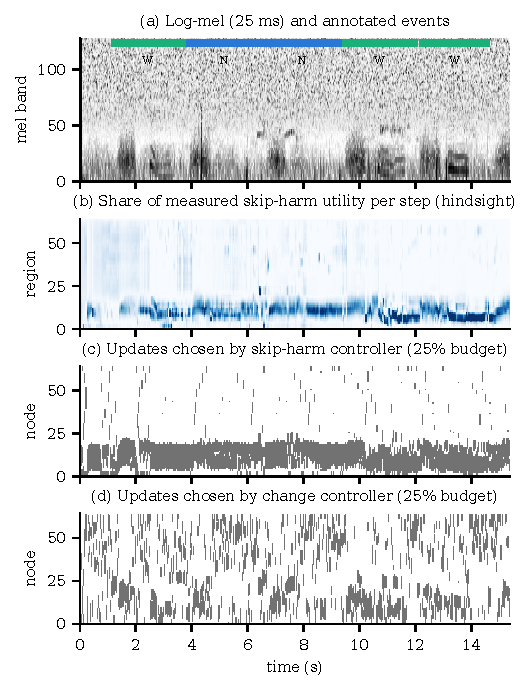
\includegraphics[width=0.72\textwidth]{figures/example.pdf}
\caption{Example 2024 test recording at a 25\% budget (seed 0). (a) Log-mel spectrogram with the annotated events (bars; W: wheeze, N: normal). (b) Each region's share of the measured skip-harm utility per step. (c) Nodes updated (dark) by our controller. (d) Nodes updated by the change-trained controller.}
\label{fig:example}
\end{figure}

\DIFaddbegin \paragraph*{\DIFadd{Why does our end-to-end gate fall short?}}
\label{sec:why-two-stage}
\DIFadd{Three observations explain the gap to the end-to-end gate in preservation. First, its training signal is weak, or at least hard to exploit with the straight-through estimator we used. The task loss of the end-to-end gate does not decrease during training (mean 1.220 in the first epoch and 1.262 in the last; 1.208 and 1.368 for the graph GRU), although the Gumbel noise is annealed (for the graph GRU it falls for two to three epochs and then rises as the noise is reduced; as for our controller, we evaluate the final epoch). The straight-through estimator only reports how the loss would change for an infinitesimally larger inclusion of each node, while the actual selection is discrete and budget-exact: adding one region forces another one out. Second, the gate's scores are poor estimates of what a skip costs. They rank regions by measured skip-harm utility with Spearman 0.24, against 0.63 for our controller. Third, the supervision differs in density. The counterfactual target gives every one of the 64 regions a regression label at every step, while the end-to-end gate receives one scalar loss per crop, distributed over all selections of all steps through back-propagation in time. The two-stage design trades exactness of the objective (a one-step surrogate instead of the task loss) for a dense, low-variance learning signal. Against a gate trained on frozen weights with an untuned schedule, this trade pays off in preservation; a jointly trained or more carefully tuned gate could narrow the gap.

}

\paragraph*{\DIFadd{Is a one-step target enough?}}
\label{sec:multistep}
\DIFadd{The utility target looks one step ahead, while a skipped state can affect later outputs. Table~\ref{tab:multistep} compares rankings with the measured multi-step harm. A skip does have lasting effects: the harm summed over 1\,s after a single skip is 13.6 times the harm in the step of the skip (median). The }\emph{\DIFadd{ranking}} \DIFadd{of regions, however, is stable. The one-step utility ranks regions by their 1\,s harm with Spearman 0.72, and by the harm of holding a region for 25 consecutive steps with 0.64. The trained controller's correlation does not degrade with the horizon (0.58 at one step and 0.61 for 25-step holds), while the change head stays low (0.26 and 0.16). The graph-GRU cell shows the same pattern at a higher level (one-step utility 0.73 and controller 0.82 for 25-step holds, change head 0.09). Since the selection only needs the ranking, the one-step proxy is sufficient here; a multi-step target would preserve most of its ranking. The test holds one region while all others are updated. In deployment at 25\%, about three quarters of the states are stale at once and can stay stale for up to the refresh threshold, a joint-staleness regime that this test does not cover.

}

\multisteptable

\paragraph*{\DIFadd{Contraction and the bound}}
\label{sec:lip}
\DIFadd{Table~\ref{tab:lipschitz} checks Proposition~\ref{prop:bound} on real trajectories. Although nothing in training enforces it, the learned transition mostly contracts the gap between the full and selective trajectories: at 25\%, the median measured secant ratio $\hat\gamma_t$ (over steps with $e_{t-1}>0$) is 0.970, and 99.2\% of the steps have $\hat\gamma_t<1$ (99th percentile 1.000). On a few steps, however, the measured ratio exceeds one (maximum 1.82). Because these ratios are measured in the proposition's norm, no uniform contraction factor $\gamma<1$ can hold for all sampled pairs of states, and only the time-varying recurrence applies. Evaluated with $\hat\gamma_t$, that recurrence holds by construction, so the check is a numerical consistency check and an assessment of tightness rather than evidence for the assumption; it is loose (median state error 3.10 against a bound of 11.9). As a separate diagnostic, the local Jacobian has a median spectral norm of 1.29 in the Euclidean norm of the whole state. This norm differs from the proposition's $\|\cdot\|_{\infty,2}$, so a value above one does not by itself rule out contraction in the proposition's norm; together with the secant ratios, it suggests that the contraction is a property of the observed trajectories, as for locally contractive recurrent networks~\mbox{%DIFAUXCMD
\cite{mitarchuk2024length}}\hskip0pt%DIFAUXCMD
, rather than a uniform property of the cell. The link to the output is weak: the readout ratio is only 0.142 (median; 99th percentile 0.489, an empirical stand-in for $L_R$ in Eq.~(\ref{eq:readout})), and the state error and the frame KL divergence are nearly uncorrelated across steps (Spearman 0.05). Most of the state error lies in directions the readout ignores. This is the empirical reason for training the controller on the output-level skip-harm utility instead of on a state-level quantity such as the representation change.

}

\liptable

\subsection{\DIFadd{Generality: Cells, Topology and Dataset (RQ3)}}
\label{sec:generality}
\DIFadd{The selection method makes no assumption about the cell, the graph or the data. We test it in three ways: with a different cell, with a different graph topology, and on a second dataset.

}

\DIFaddend \ifgg
\DIFdelbegin \subsection{\DIFdel{Transfer to Another Graph Cell (RQ3)}}
%DIFAUXCMD
\addtocounter{subsection}{-1}%DIFAUXCMD
\DIFdelend \DIFaddbegin \paragraph*{\DIFadd{Another cell}}
\DIFaddend \label{sec:gg}
We repeated the selection pipeline, with the same hyperparameters, on the plain graph-GRU cell, the \DIFdelbegin \DIFdel{strongest }\DIFdelend \DIFaddbegin \DIFadd{most accurate }\DIFaddend full-update backbone \DIFaddbegin \DIFadd{on the chain graph }\DIFaddend (Section~\ref{sec:backbones}). Table~\ref{tab:policygg} shows the same picture. At 25\%, the skip-harm controller preserves $F_{\mathrm{pres}}=0.712$, against 0.210 for the change objective, 0.167 for periodic and 0.158 for random. It wins in every seed, by 0.48--0.55 over the change objective. This cell relies even more on its state (preservation 0.064 without updates), and its utility is even more concentrated (95.3\% in the top quarter). Against the annotations, event $F$ at 25\% is 0.120 versus 0.128 with full updates (\ensuremath{-}0.0081 [\ensuremath{-}0.0119, \ensuremath{-}0.0043]). Non-inferiority is therefore narrowly missed at 25\% on the 2024 set, but it holds on the 2025 release and at 50\%. The advantage of the skip-harm target is thus not specific to the AGN-Net cell. \DIFaddbegin \DIFadd{The end-to-end gate is particularly unreliable on this cell: at 25\% it preserves 0.358 on average, below our controller in every seed by 0.16--0.54.

}\DIFaddend 

\policytable{tables/policy_gg_C.tex}{Selection policies for the plain graph-GRU cell (same setup as Table~\ref{tab:policy}).}{tab:policygg}
\fi

\DIFaddbegin \paragraph*{\DIFadd{Another topology}}
\label{sec:harmonic}
\DIFadd{The harmonic edges (Section~\ref{sec:method}) let one update pass evidence between a fundamental and its overtones. Table~\ref{tab:policyh} shows the selection policies for the AGN-Net cell on this harmonic graph. The skip-harm controller stays well ahead of the change objective and random selection: at 25\%, it preserves $F_{\mathrm{pres}}=0.554$, against 0.327 for the change objective and 0.212 for random selection, and it is better than the change objective in 3 of 3 seeds. Absolute preservation is lower than on the chain graph (0.775), possibly because regions on the harmonic graph contain up to 9 nodes, so a fixed budget is spent in fewer and coarser regions, and because this model depends more on its state (preservation 0.036 without graph updates, against 0.163 on the chain). The hindsight oracle falls as well (0.625), but our controller is further from it than on the chain graph, so its predictions transfer less well to the larger regions; at 25\%, event $F$ against the annotations is therefore not non-inferior on this graph (}\ensuremath{-}\DIFadd{0.0144 }[\ensuremath{-}\DIFadd{0.0192, }\ensuremath{-}\DIFadd{0.0092}]\DIFadd{). The harmonic edges do help the cell itself. With full updates, the AGN-Net cell on the harmonic graph reaches event $F=0.139$ on the 2024 test set, against 0.087 on the chain (Section~\ref{sec:backbones}), and it is far more consistent across seeds: the chain-graph cell had one strong and two weak seeds, whereas all three harmonic seeds are close to the plain graph GRU (0.133). The harmonic topology thus mainly removes the instability of the AGN-Net cell rather than surpassing the graph GRU, whose segment-based adventitious score remains higher (0.301 vs.\ 0.216). Adventitious event $F$ does not improve, and the harmonic graph is also denser (up to 8 neighbours instead of 4, and several low-frequency harmonic edges join nodes only 3--6 positions apart), so the gain cannot be attributed specifically to propagation between harmonics. A learned or adaptive topology is a natural extension, and the controller applies to it unchanged.

}

\policytable{tables/policy_h_C.tex}{Selection policies for the AGN-Net cell on the harmonic graph (same setup as Table~\ref{tab:policy}).}{tab:policyh}

\paragraph*{\DIFadd{Another dataset}}
\label{sec:hflung}
\DIFadd{Table~\ref{tab:hflung} repeats the comparison on HF\_Lung\_V1, with adult patients, two recording devices and a different label set. The picture is the same. At 25\%, the skip-harm controller preserves $F_{\mathrm{pres}}=0.736$ with the AGN-Net cell, against 0.638 for the change objective and 0.330 for random selection (bootstrap difference to random 0.405 }[\DIFadd{0.359, 0.441}]\DIFadd{), and 0.744 against 0.494 and 0.314 with the graph GRU. The controller is better than the change objective, periodic refresh and random selection in every seed and at every budget, for both cells. The ranking diagnostics agree: the controller ranks regions by measured utility with Spearman 0.82 on HF\_Lung, whereas acoustic change correlates only weakly (0.20), and utility is again concentrated (92.2\% in the top quarter of regions). Against the annotations, absolute scores are higher than on SPRSound (full-update event $F$ 0.232). At 25\%, the selective model's event $F$ is 0.225 (}\ensuremath{-}\DIFadd{0.0064 }[\ensuremath{-}\DIFadd{0.0125, }\ensuremath{-}\DIFadd{0.0012}]\DIFadd{), so non-inferiority is narrowly missed at 25\%; it holds at 50\% (0.0017 }[\ensuremath{-}\DIFadd{0.0001, 0.0044}]\DIFadd{). With the graph GRU the loss at 25\% is larger (}\ensuremath{-}\DIFadd{0.0139 }[\ensuremath{-}\DIFadd{0.0217, }\ensuremath{-}\DIFadd{0.0087}]\DIFadd{), and non-inferiority again holds at 50\%. The concentration of utility in a few frequency regions, and the controller's advantage, are therefore not specific to the paediatric data or to one recording device.

}

\hfltable

\DIFaddend \subsection{Ablation Study (RQ4)}
\paragraph*{Training target} All three utility targets clearly beat the change target (Table~\ref{tab:policy}). The hold-only target is about as good as the full two-endpoint target: slightly better at 12.5\% (0.559 vs.\ 0.552) and slightly worse at 25\% (0.768 vs.\ 0.775). Removing the label term costs 0.069 $F_{\mathrm{pres}}$ at 25\% (bootstrap estimate). What matters most is that the target measures the effect on the output.

\paragraph*{Refresh rule} Forcing refreshes of stale states uses part of the budget. Without it, $F_{\mathrm{pres}}$ is 0.582 instead of 0.552 at 12.5\% and 0.770 instead of 0.775 at 25\%. On these short recordings (at most 15\,s) the rule costs a little at the smallest budget \DIFaddbegin \DIFadd{for this cell, and more for the graph GRU (0.350 without refresh instead of 0.305 at 12.5\%, 0.728 instead of 0.712 at 25\%).

}

\paragraph*{\DIFadd{Refresh on long streams}}
\label{sec:long}
\DIFadd{Table~\ref{tab:long} evaluates the refresh rule where it should matter, on continuous 60--120\,s patient streams. The effects are small and vary between seeds; these tests use the AGN-Net cell on the chain graph. At 25\%, refresh helps on average (strongly in one seed and negligibly in a second, while in the third it lowers preservation by about 0.02): preservation is 0.771 without refresh and 0.793 with the 2\,s rule, and without refresh the frame-level agreement with the full model drifts down later in the stream (0.967 in the first 15\,s, 0.960 after 30\,s), whereas with the 2\,s rule it stays level (0.968 and 0.967). At 12.5\%, the fixed 2\,s threshold costs preservation (0.573 vs.\ 0.595 without refresh), because a full refresh cycle then uses up to 16\% of the budget. No fixed threshold is best at every budget: the short threshold $A{=}25$ loses 0.530 against 0.595 at 12.5\%, and no refresh loses at 25\%. The budget-adaptive threshold $A(b)=\lceil 12.5/b\rceil$ stays within 0.01 of the best rule at every budget (0.585, 0.793 and 0.916 at 12.5\%, 25\% and 50\%), as does the fixed $A{=}100$, and the 2025 release shows the same pattern. We therefore recommend a budget-dependent threshold such as $A(b)$ for deployment; on streams of hours rather than minutes, where staleness can grow much further, the refresh rule may matter more than in our tests}\DIFaddend .

\DIFdelbegin \DIFdel{Its benefit, protection against arbitrarily old states, would only appear on longer streams .

}\DIFdelend 

\DIFaddbegin \longtable

\DIFaddend \paragraph*{Selective fine-tuning} Before fine-tuning (stage-A weights, Table~\ref{tab:policyA}), preservation is lower for every policy (0.533 for ours and 0.352 for random at 25\%). The utility heads are still best on average, but the ordering varies across seeds. Fine-tuning under selective rollouts with distillation raises our controller to 0.775, while random rises only to 0.414. Part of this gain may come from the fine-tuning mixture, which samples the utility-based policies more often.

\paragraph*{Fresh-feature path} Without the fresh features in the readout (Table~\ref{tab:policynf}), the model cannot react to the current chunk unless states are updated. Selection therefore matters even more: at 25\%, our controller preserves 0.608, against 0.198 for random. The fresh path makes selective inference more forgiving, but our advantage does not depend on it.

\policytable{tables/policy_A.tex}{Selection policies on the stage-A weights (before selective fine-tuning). Columns, bold and $^\dagger$ as in Table~\ref{tab:policy}.}{tab:policyA}
\policytable{tables/policy_nf_C.tex}{Selection policies for the model without the fresh-feature path in the readout. Columns, bold and $^\dagger$ as in Table~\ref{tab:policy}.}{tab:policynf}

\runtimetable

\subsection{Efficiency (RQ5)}
\label{sec:h3}
Table~\ref{tab:runtime} and Figure~\ref{fig:runtime} report streaming latency on one CPU core. All configurations run far faster than real time: a full update takes 2.76\,ms per 40\,ms chunk in the NumPy runtime, of which 1.45\,ms is the graph update. With our controller at 25\%, the graph update drops to 0.71\,ms, but the controller adds 0.42\,ms. The net speedup is 1.22$\times$ at 12.5\%, 1.14$\times$ at 25\% and 1.02$\times$ at 50\%. Random and periodic selection are faster (1.32$\times$ and 1.35$\times$ at 25\%) because their scores are almost free, but they preserve far fewer events. Removing the graph entirely gives 2.21$\times$, an upper bound on the possible gain. In the PyTorch runtime, operator-launch overhead dominates the small graph, and selective inference is slower than full updating (0.88$\times$). The efficiency gain is therefore real but modest, and it depends on a lean runtime and on keeping the controller cheap.

\DIFaddbegin \paragraph*{\DIFadd{How the overhead scales}} \DIFadd{The overhead is large here because our cell is small: at $d{=}96$, the controller costs 60.4\% of the time saved by skipping 75\% of the graph update. The controller's arithmetic grows only linearly with the state size (through its input), whereas the cell's parameters and arithmetic grow quadratically with $d$ and linearly with the number of layers. Table~\ref{tab:scaling} shows the consequence. With $d{=}384$ the controller's share falls to 19.1\%, and with $d{=}768$ to 8.9\% (7.1\% with four layers), and the speedup of the graph stage at 25\% rises from 1.25$\times$ to 1.82$\times$. The speedup stays below the ideal $4\times$ and levels off near $1.8\times$: in this runtime, updating a quarter of the nodes still takes about half the time of the full graph update at every size (presumably because the small per-call matrix products are dominated by loading the $d\times d$ weights rather than by arithmetic; we did not profile this), so a smaller controller share alone does not approach the ideal. On embedded accelerators (digital signal processors, DSPs, or neural processing units, NPUs), two further effects matter that we did not measure: the controller is a small dense network that maps well onto such hardware, but sparse gather/scatter of a changing node set is less efficient there than dense computation, so a block-structured selection (e.g., fixed groups of regions) may be needed to turn skipped updates into energy savings.

}

\scaltable

\DIFaddend \begin{figure}[H]
\centering
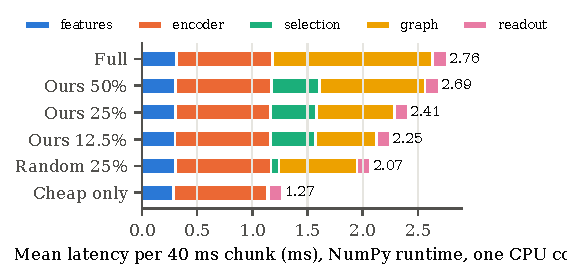
\includegraphics[width=0.8\textwidth]{figures/runtime_numpy.pdf}
\caption{Per-chunk latency by stage in the NumPy runtime (one CPU core, mean over seeds).}
\label{fig:runtime}
\end{figure}

\archtable

\subsection{Comparison of Full-Update Backbones}
\label{sec:backbones}
Table~\ref{tab:arch} compares the backbones when every node is updated at every step (stage-A weights). Graph-structured state helps: the plain graph GRU \DIFdelbegin \DIFdel{is the best model, with }\DIFdelend \DIFaddbegin \DIFadd{reaches }\DIFaddend event $F=0.133$ and \DIFaddbegin \DIFadd{the best }\DIFaddend seg-adv-\DIFdelbegin \DIFdel{$F=0.301$ }\DIFdelend \DIFaddbegin \DIFadd{$F$ (0.301) }\DIFaddend on the 2024 set, ahead of the GRU, the TCN and memoryless pooling. \DIFdelbegin \DIFdel{Our }\DIFdelend \DIFaddbegin \DIFadd{On the chain graph, our }\DIFaddend AGN-Net cell \DIFdelbegin \DIFdel{, however, }\DIFdelend is not better than the plain graph GRU\DIFdelbegin \DIFdel{. Its }\DIFdelend \DIFaddbegin \DIFadd{; on the harmonic graph it reaches a similar event $F$ (0.139) but a lower seg-adv-$F$ (0.216). On the chain graph its }\DIFaddend mean event $F$ is 0.087, with a large variance across seeds: one seed is \DIFdelbegin \DIFdel{the best model }\DIFdelend \DIFaddbegin \DIFadd{among the best single runs }\DIFaddend in the study, while the other two are among the weakest. Absolute scores are low for all models, mainly because of the annotation shift between training and test data. Offline detectors designed for this benchmark, such as EZhouNet~\cite{chu2026ezhounet}, report higher event-level scores. Our claims concern selective computation relative to a given model, not state-of-the-art detection accuracy.

\section{Conclusion}
\label{sec:conclusion}

We studied how a streaming respiratory sound detector can decide which of its expensive state updates to skip. \DIFdelbegin \DIFdel{Our }\DIFdelend \DIFaddbegin \DIFadd{The }\DIFaddend model keeps a persistent graph of frequency regions, observes every chunk with a cheap encoder, and updates only a budget-limited set of regions chosen by a learned controller. The key change from AGN-Net is the training target of the controller: it predicts how much skipping a region's update would change the model's output, not how much the region's representation will change. \DIFdelbegin \DIFdel{On SPRSound}\DIFdelend \DIFaddbegin \DIFadd{With the same number of node updates}\DIFaddend , this controller preserves the full-update model's detections far better than random, periodic, energy-based \DIFdelbegin \DIFdel{, change-based and AGN-Net-style selection}\DIFdelend \DIFaddbegin \DIFadd{and change-based selection, and better than a gate of the same size trained on the task loss on top of the frozen model, }\DIFaddend at every budget \DIFdelbegin \DIFdel{. }\DIFdelend \DIFaddbegin \DIFadd{and in every seed. The advantage holds for two cells, and the advantage over change-based and random selection also holds for a harmonic graph topology and on a second, adult dataset, so it is a property of the selection method rather than of one backbone. }\DIFaddend With a quarter of the graph updates, \DIFdelbegin \DIFdel{its }\DIFdelend \DIFaddbegin \DIFadd{the AGN-Net cell's }\DIFaddend event F against the annotations \DIFaddbegin \DIFadd{on SPRSound }\DIFaddend is non-inferior to full updating\DIFdelbegin \DIFdel{. Analysis shows }\DIFdelend \DIFaddbegin \DIFadd{; in the other settings it is missed at 25\% on the 2024 set or on HF\_Lung (narrowly for the graph GRU on SPRSound and the AGN-Net cell on HF\_Lung, more clearly for the harmonic graph and for the graph GRU on HF\_Lung) and holds at 50\% in all settings. The analyses explain }\DIFaddend why: skip-harm utility is \DIFaddbegin \DIFadd{concentrated in a few regions and }\DIFaddend predictable from information available at inference time\DIFdelbegin \DIFdel{and concentrated in a few regions , whereas spectral change is a misleading signal. Retraining the same recipe on a plain graph-GRU cell gives the same ordering, so the advantage is not specific to the AGN-Net cell. It is }\DIFdelend \DIFaddbegin \DIFadd{, the one-step target ranks regions well by their multi-step harm, and the state error that a selective update causes lies mostly in directions the readout ignores, which a state-level objective cannot see. The advantage is }\DIFaddend most plausibly due to the training target, although we tested only two \DIFdelbegin \DIFdel{graph cellson one dataset}\DIFdelend \DIFaddbegin \DIFadd{cells, two graph topologies and two datasets}\DIFaddend .

The work has limitations. \DIFdelbegin \DIFdel{All experiments use one paediatric dataset, whose }\DIFdelend \DIFaddbegin \DIFadd{On SPRSound the }\DIFaddend test releases follow a different annotation style\DIFdelbegin \DIFdel{. Absolute detection scores are therefore }\DIFdelend \DIFaddbegin \DIFadd{, so absolute event scores are }\DIFaddend low for every model \DIFdelbegin \DIFdel{, and they are }\DIFdelend \DIFaddbegin \DIFadd{and }\DIFaddend below those of offline detectors built for this benchmark\DIFaddbegin \DIFadd{; boundary-tolerant metrics show that much of the low strict-collar score comes from boundary conventions}\DIFaddend . The AGN-Net cell was not a better detector than a plain graph GRU\DIFaddbegin \DIFadd{; harmonic graph edges made it comparable in event F and much more stable, but it stayed below the graph GRU on the adventitious metrics, and on HF\_Lung the AGN-Net cell occasionally diverged during training}\DIFaddend . The end-to-end speedup \DIFdelbegin \DIFdel{was }\DIFdelend \DIFaddbegin \DIFadd{at our model size is }\DIFaddend modest (1.14$\times$ at 25\% of the updates \DIFdelbegin \DIFdel{) and appeared only }\DIFdelend in a lightweight runtime, \DIFdelbegin \DIFdel{since the controller itself costs about half }\DIFdelend \DIFaddbegin \DIFadd{none in PyTorch eager mode), because the controller costs a large part }\DIFaddend of the time it saves\DIFdelbegin \DIFdel{. Finally, }\DIFdelend \DIFaddbegin \DIFadd{; the overhead shrinks for larger cells, but }\DIFaddend we did not \DIFdelbegin \DIFdel{compare with gates trained end to end on the task loss. }\DIFdelend \DIFaddbegin \DIFadd{measure on embedded hardware. The skip-harm target is a one-step proxy whose ranking we tested for one stale region at a time, not for many regions stale together; the end-to-end gate was trained on a frozen backbone with untuned settings; and our longest streams last two minutes, so the refresh rule was tested only where staleness stays moderate. Proposition~\ref{prop:bound} is conditional, and its link to the output is loose.

}\DIFaddend 

Future work includes \DIFdelbegin \DIFdel{a cheaper controller, multi-step utility targets, comparison with end-to-end trained gates, evaluation on other datasets and devices, and deployment on embedded hardware }\DIFdelend \DIFaddbegin \DIFadd{cheaper or amortised controllers, learned and adaptive graph topologies, block-structured selection for embedded accelerators }\DIFaddend where sparse updates translate into energy savings\DIFdelbegin \DIFdel{. Code, data manifests, the patient-disjoint split and all }\DIFdelend \DIFaddbegin \DIFadd{, and evaluation on long-term wearable recordings. All code, logs, }\DIFaddend per-recording results \DIFdelbegin \DIFdel{will be released with the paper}\DIFdelend \DIFaddbegin \DIFadd{and trained weights are public at }\url{https://github.com/redwanUGA/event-aware-agn-net}\DIFaddend .


%=================================================================
\vspace{6pt}

\funding{This research received no external funding.}

\DIFdelbegin %DIFDELCMD < \institutionalreview{Ethical review and approval were not required for this study because it is a secondary analysis of the publicly available, de-identified SPRSound database~\cite{zhang2022sprsound,sprsound2025repo}; no new data were collected and no participants were contacted.}
%DIFDELCMD < %%%
\DIFdelend \DIFaddbegin \institutionalreview{Ethical review and approval were not required for this study because it is a secondary analysis of the publicly available, de-identified SPRSound~\cite{zhang2022sprsound,sprsound2025repo} and HF\_Lung\_V1~\cite{hsu2021benchmarking} databases; no new data were collected and no participants were contacted.}
\DIFaddend 

\informedconsent{Not applicable. Only publicly available, de-identified data were analysed, and no participants were contacted.}

\DIFdelbegin %DIFDELCMD < \dataavailability{The SPRSound data analysed in this study are publicly available at \url{https://github.com/SJTU-YONGFU-RESEARCH-GRP/SPRSound}~\cite{zhang2022sprsound,sprsound2025repo}. The code, data manifests, patient-disjoint split and per-recording results that support the findings are available from the author on request during peer review and will be deposited in a public repository upon publication.}
%DIFDELCMD < %%%
\DIFdelend \DIFaddbegin \dataavailability{The SPRSound data analysed in this study are publicly available at \url{https://github.com/SJTU-YONGFU-RESEARCH-GRP/SPRSound}~\cite{zhang2022sprsound,sprsound2025repo}. The HF\_Lung\_V1 data are publicly available at \url{https://gitlab.com/techsupportHF/HF_Lung_V1}~\cite{hsu2021benchmarking}. The complete code, configurations, job lists, training and evaluation logs, per-recording results, trained weights and data-split manifests that support the findings are publicly available at \url{https://github.com/redwanUGA/event-aware-agn-net}.}
\DIFaddend 

\DIFdelbegin %DIFDELCMD < \acknowledgments{The author acknowledges the Georgia Advanced Computing Resource Center (GACRC) at the University of Georgia for providing the computing resources used in this study. During the preparation of this study, the author used Claude Opus~5.5 (Anthropic) for the purposes of writing experiment and analysis code, running the experiments, analysing the results and drafting the manuscript text. The author has reviewed and edited the output and takes full responsibility for the content of this publication.}
%DIFDELCMD < %%%
\DIFdelend \DIFaddbegin \acknowledgments{The author acknowledges the Georgia Advanced Computing Resource Center (GACRC) at the University of Georgia for providing the computing resources used in this study. During the preparation of this study, the author used Claude Opus~5.5 (Anthropic) for the purposes of proposing the detailed experimental protocol, writing experiment and analysis code, running the experiments, drafting Proposition~1 and its proof, drafting the interpretation of the results and drafting the manuscript text (see Section~\ref{sec:genai} and Table~\ref{tab:genai}). The author has reviewed and edited the output and takes full responsibility for the content of this publication.}
\DIFaddend 

\conflictsofinterest{The author declares no conflicts of interest.}

\DIFdelbegin %DIFDELCMD < \abbreviations{Abbreviations}{%
%DIFDELCMD < The following abbreviations are used in this manuscript:\\
%DIFDELCMD < 

%DIFDELCMD < \noindent
%DIFDELCMD < \begin{tabular}{@{}ll}
%DIFDELCMD < CE & Cross-entropy\\
%DIFDELCMD < CNN & Convolutional neural network\\
%DIFDELCMD < CPU & Central processing unit\\
%DIFDELCMD < DCASE & Detection and Classification of Acoustic Scenes and Events\\
%DIFDELCMD < ELU & Exponential linear unit\\
%DIFDELCMD < GCN & Graph convolutional network\\
%DIFDELCMD < GELU & Gaussian-error linear unit\\
%DIFDELCMD < GPU & Graphics processing unit\\
%DIFDELCMD < GRU & Gated recurrent unit\\
%DIFDELCMD < HS & Harmonic score\\
%DIFDELCMD < KL & Kullback--Leibler (divergence)\\
%DIFDELCMD < LN & Layer normalization\\
%DIFDELCMD < MLP & Multilayer perceptron\\
%DIFDELCMD < RNN & Recurrent neural network\\
%DIFDELCMD < TCN & Temporal convolutional network
%DIFDELCMD < \end{tabular}
%DIFDELCMD < }
%DIFDELCMD < %%%
\DIFdelend \DIFaddbegin \abbreviations{Abbreviations}{%
The following abbreviations are used in this manuscript:\\

\noindent
\begin{tabular}{@{}ll}
CE & Cross-entropy\\
CNN & Convolutional neural network\\
CPU & Central processing unit\\
DCASE & Detection and Classification of Acoustic Scenes and Events\\
DSP & Digital signal processor\\
ELU & Exponential linear unit\\
GCN & Graph convolutional network\\
GELU & Gaussian-error linear unit\\
GPU & Graphics processing unit\\
GRU & Gated recurrent unit\\
HS & Harmonic score\\
KL & Kullback--Leibler (divergence)\\
LN & Layer normalization\\
MLP & Multilayer perceptron\\
NPU & Neural processing unit\\
RNN & Recurrent neural network\\
TCN & Temporal convolutional network
\end{tabular}
}
\DIFaddend 

%=================================================================
\begin{adjustwidth}{-\extralength}{0cm}
\reftitle{References}
\begin{thebibliography}{999}

\bibitem[Bardou et~al.(2018)Bardou, Zhang, and Ahmad]{bardou2018lung}
Bardou, D.; Zhang, K.; Ahmad, S.M.
\newblock Lung sounds classification using convolutional neural networks.
\newblock {\em Artificial Intelligence in Medicine} {\bf 2018}, {\em
  88},~58--69.
\newblock {\url{https://doi.org/10.1016/j.artmed.2018.04.008}}.

\bibitem[Petmezas et~al.(2022)Petmezas, Cheimariotis, Stefanopoulos, Rocha,
  Paiva, Katsaggelos, and Maglaveras]{petmezas2022automated}
Petmezas, G.; Cheimariotis, G.A.; Stefanopoulos, L.; Rocha, B.; Paiva, R.P.;
  Katsaggelos, A.K.; Maglaveras, N.
\newblock Automated Lung Sound Classification Using a Hybrid {CNN-LSTM} Network
  and Focal Loss Function.
\newblock {\em Sensors} {\bf 2022}, {\em 22},~1232.
\newblock {\url{https://doi.org/10.3390/s22031232}}.

\bibitem[Niizumi et~al.(2025)Niizumi, Takeuchi, Yasuda, Nguyen, Ohishi, and
  Harada]{niizumi2025towards}
Niizumi, D.; Takeuchi, D.; Yasuda, M.; Nguyen, B.T.; Ohishi, Y.; Harada, N.
\newblock Towards Pre-training an Effective Respiratory Audio Foundation Model.
\newblock In Proceedings of the Interspeech 2025,  2025, pp. 998--1002.
\newblock {\url{https://doi.org/10.21437/Interspeech.2025-84}}.

\bibitem[Neil et~al.(2017)Neil, Lee, Delbruck, and Liu]{neil2017delta}
Neil, D.; Lee, J.H.; Delbruck, T.; Liu, S.C.
\newblock Delta Networks for Optimized Recurrent Network Computation.
\newblock In Proceedings of the 34th International Conference on Machine
  Learning (ICML); Precup, D.; Teh, Y.W., Eds., Sydney, Australia,  2017;
  Vol.~70, {\em Proceedings of Machine Learning Research}, pp. 2584--2593.

\bibitem[Campos et~al.(2018)Campos, Jou, Gir{\'o}-i Nieto, Torres, and
  Chang]{campos2018skip}
Campos, V.; Jou, B.; Gir{\'o}-i Nieto, X.; Torres, J.; Chang, S.F.
\newblock Skip {RNN}: Learning to Skip State Updates in Recurrent Neural
  Networks.
\newblock In Proceedings of the International Conference on Learning
  Representations (ICLR),  2018.

\bibitem[Jernite et~al.(2017)Jernite, Grave, Joulin, and
  Mikolov]{jernite2017variable}
Jernite, Y.; Grave, E.; Joulin, A.; Mikolov, T.
\newblock Variable Computation in Recurrent Neural Networks.
\newblock In Proceedings of the International Conference on Learning
  Representations (ICLR),  2017.

\bibitem[Seo et~al.(2018{\natexlab{a}})Seo, Min, Farhadi, and
  Hajishirzi]{seo2018neural}
Seo, M.; Min, S.; Farhadi, A.; Hajishirzi, H.
\newblock Neural Speed Reading via {Skim-RNN}.
\newblock In Proceedings of the International Conference on Learning
  Representations (ICLR),  2018.

\bibitem[Seo et~al.(2018{\natexlab{b}})Seo, Defferrard, Vandergheynst, and
  Bresson]{seo2018structured}
Seo, Y.; Defferrard, M.; Vandergheynst, P.; Bresson, X.
\newblock Structured Sequence Modeling with Graph Convolutional Recurrent
  Networks.
\newblock In Proceedings of the Neural Information Processing (ICONIP 2018).
  Springer, Cham,  2018, Vol. 11301, {\em Lecture Notes in Computer Science},
  pp. 362--373.
\newblock {\url{https://doi.org/10.1007/978-3-030-04167-0_33}}.

\bibitem[Rossi et~al.(2020)Rossi, Chamberlain, Frasca, Eynard, Monti, and
  Bronstein]{rossi2020temporal}
Rossi, E.; Chamberlain, B.; Frasca, F.; Eynard, D.; Monti, F.; Bronstein, M.
\newblock Temporal Graph Networks for Deep Learning on Dynamic Graphs.
\newblock {\em arXiv} {\bf 2020}.
\newblock {\url{https://doi.org/10.48550/arXiv.2006.10637}}.

\bibitem[Islam et~al.(2026)Islam, Sadatian~Moghaddam, and
  Arpinar]{islam2026agnnet}
Islam, M.R.; Sadatian~Moghaddam, P.; Arpinar, I.B.
\newblock {AquaGraph} and {AGN-Net}: A Biologically Inspired Framework for
  Scalable and Adaptive Graph Neural Networks.
\newblock {\em IEEE Access} {\bf 2026}, {\em 14},~150366--150382.
\newblock {\url{https://doi.org/10.1109/ACCESS.2026.3737793}}.

\bibitem[Rocha et~al.(2019)Rocha, Filos, Mendes, Serbes, Ulukaya, Kahya,
  Jakovljevi{\'c}, Turukalo, Vogiatzis, Perantoni, Kaimakamis, Natsiavas,
  Oliveira, J{\'a}come, Marques, Maglaveras, Paiva, Chouvarda, and
  de~Carvalho]{rocha2019open}
Rocha, B.M.; Filos, D.; Mendes, L.; Serbes, G.; Ulukaya, S.; Kahya, Y.P.;
  Jakovljevi{\'c}, N.; Turukalo, T.L.; Vogiatzis, I.M.; Perantoni, E.;  et~al.
\newblock An open access database for the evaluation of respiratory sound
  classification algorithms.
\newblock {\em Physiological Measurement} {\bf 2019}, {\em 40},~035001.
\newblock {\url{https://doi.org/10.1088/1361-6579/ab03ea}}.

\bibitem[Zhang et~al.(2022{\natexlab{a}})Zhang, Zhang, Yuan, Huang, Zhang,
  Zhang, Lv, Lin, Wang, Liu, Tang, Wang, Ma, Liu, Yuan, Zhou, Zhao, Li, Yin,
  Zhao, Wang, and Lian]{zhang2022sprsound}
Zhang, Q.; Zhang, J.; Yuan, J.; Huang, H.; Zhang, Y.; Zhang, B.; Lv, G.; Lin,
  S.; Wang, N.; Liu, X.;  et~al.
\newblock {SPRSound}: Open-Source {SJTU} Paediatric Respiratory Sound Database.
\newblock {\em IEEE Transactions on Biomedical Circuits and Systems} {\bf
  2022}, {\em 16},~867--881.
\newblock {\url{https://doi.org/10.1109/TBCAS.2022.3204910}}.

\bibitem[Zhang et~al.(2022{\natexlab{b}})Zhang, Zhang, Yuan, Huang, Zhang,
  Zhang, Lv, Lin, Wang, Liu, Tang, Wang, Ma, Liu, Yuan, Zhou, Zhao, Li, Yin,
  Zhao, Wang, and Lian]{zhang2022grand}
Zhang, Q.; Zhang, J.; Yuan, J.; Huang, H.; Zhang, Y.; Zhang, B.; Lv, G.; Lin,
  S.; Wang, N.; Liu, X.;  et~al.
\newblock Grand Challenge on Respiratory Sound Classification for {SPRSound}
  Dataset.
\newblock In Proceedings of the 2022 IEEE Biomedical Circuits and Systems
  Conference (BioCAS), Taipei, Taiwan,  2022; pp. 213--217.
\newblock {\url{https://doi.org/10.1109/BioCAS54905.2022.9948551}}.

\bibitem[Zhang et~al.(2024)Zhang, Chen, Yuan, Zhang, Yuan, Huang, Zhang, Pan,
  Jiang, Zhao, Li, Yin, Zhao, Wang, and Lian]{zhang2024meta}
Zhang, Q.; Chen, C.; Yuan, S.; Zhang, J.; Yuan, J.; Huang, H.; Zhang, Y.; Pan,
  R.; Jiang, X.; Zhao, J.;  et~al.
\newblock Meta: Data Compression and Event Detection Grand Challenge 2024 With
  {SPRSound} Dataset.
\newblock {\em IEEE Data Descriptions} {\bf 2024}, {\em 1},~122--130.
\newblock {\url{https://doi.org/10.1109/IEEEDATA.2024.3477390}}.

\bibitem[Hsu et~al.(2021)Hsu, Huang, Huang, Huang, Cheng, Chen, Hsiao, Chen,
  Chen, Lai, Hsu, Lin, Tsai, Wu, Tseng, Tseng, Chen, and
  Lai]{hsu2021benchmarking}
Hsu, F.S.; Huang, S.R.; Huang, C.W.; Huang, C.J.; Cheng, Y.R.; Chen, C.C.;
  Hsiao, J.; Chen, C.W.; Chen, L.C.; Lai, Y.C.;  et~al.
\newblock Benchmarking of eight recurrent neural network variants for breath
  phase and adventitious sound detection on a self-developed open-access lung
  sound database---{HF\_Lung\_V1}.
\newblock {\em PLOS ONE} {\bf 2021}, {\em 16},~e0254134.
\newblock {\url{https://doi.org/10.1371/journal.pone.0254134}}.

\bibitem[Hsu et~al.(2022)Hsu, Huang, Huang, Cheng, Chen, Hsiao, Chen, and
  Lai]{hsu2022progressively}
Hsu, F.S.; Huang, S.R.; Huang, C.W.; Cheng, Y.R.; Chen, C.C.; Hsiao, J.; Chen,
  C.W.; Lai, F.
\newblock A Progressively Expanded Database for Automated Lung Sound Analysis:
  An Update.
\newblock {\em Applied Sciences} {\bf 2022}, {\em 12},~7623.
\newblock {\url{https://doi.org/10.3390/app12157623}}.

\bibitem[Heitmann et~al.(2023)Heitmann, Glangetas, Doenz, Dervaux, Shama,
  Hinjos~Garcia, Benissa, Cantais, Perez, M{\"u}ller, Chavdarova,
  Ruchonnet-Metrailler, Siebert, Lacroix, Jaggi, Gervaix, Hartley, and
  {Pneumoscope Study Group}]{heitmann2023deepbreath}
Heitmann, J.; Glangetas, A.; Doenz, J.; Dervaux, J.; Shama, D.M.;
  Hinjos~Garcia, D.; Benissa, M.R.; Cantais, A.; Perez, A.; M{\"u}ller, D.;
  et~al.
\newblock {DeepBreath}---automated detection of respiratory pathology from lung
  auscultation in 572 pediatric outpatients across 5 countries.
\newblock {\em npj Digital Medicine} {\bf 2023}, {\em 6},~104.
\newblock {\url{https://doi.org/10.1038/s41746-023-00838-3}}.

\bibitem[Demir et~al.(2020{\natexlab{a}})Demir, Sengur, and
  Bajaj]{demir2020convolutional}
Demir, F.; Sengur, A.; Bajaj, V.
\newblock Convolutional neural networks based efficient approach for
  classification of lung diseases.
\newblock {\em Health Information Science and Systems} {\bf 2020}, {\em 8},~4.
\newblock {\url{https://doi.org/10.1007/s13755-019-0091-3}}.

\bibitem[Demir et~al.(2020{\natexlab{b}})Demir, Ismael, and
  Sengur]{demir2020classification}
Demir, F.; Ismael, A.M.; Sengur, A.
\newblock Classification of Lung Sounds With {CNN} Model Using Parallel Pooling
  Structure.
\newblock {\em IEEE Access} {\bf 2020}, {\em 8},~105376--105383.
\newblock {\url{https://doi.org/10.1109/ACCESS.2020.3000111}}.

\bibitem[Acharya and Basu(2020)]{acharya2020deep}
Acharya, J.; Basu, A.
\newblock Deep Neural Network for Respiratory Sound Classification in Wearable
  Devices Enabled by Patient Specific Model Tuning.
\newblock {\em IEEE Transactions on Biomedical Circuits and Systems} {\bf
  2020}, {\em 14},~535--544.
\newblock {\url{https://doi.org/10.1109/TBCAS.2020.2981172}}.

\bibitem[Crisdayanti et~al.(2024)Crisdayanti, Nam, Jung, and
  Kim]{crisdayanti2024attention}
Crisdayanti, I.A.P.A.; Nam, S.W.; Jung, S.K.; Kim, S.E.
\newblock Attention Feature Fusion Network via Knowledge Propagation for
  Automated Respiratory Sound Classification.
\newblock {\em IEEE Open Journal of Engineering in Medicine and Biology} {\bf
  2024}, {\em 5},~383--392.
\newblock {\url{https://doi.org/10.1109/OJEMB.2024.3402139}}.

\bibitem[Dong et~al.(2025)Dong, Shen, Wang, Zhang, Sun, and
  Zhang]{dong2025respiratory}
Dong, G.; Shen, Y.; Wang, J.; Zhang, M.; Sun, P.; Zhang, M.
\newblock Respiratory sounds classification by fusing the time-domain and {2D}
  spectral features.
\newblock {\em Biomedical Signal Processing and Control} {\bf 2025}, {\em
  107},~107790.
\newblock {\url{https://doi.org/10.1016/j.bspc.2025.107790}}.

\bibitem[Kim et~al.(2025)Kim, Kim, Leem, Kim, and Lee]{kim2025enhanced}
Kim, Y.; Kim, K.B.; Leem, A.Y.; Kim, K.; Lee, S.H.
\newblock Enhanced Respiratory Sound Classification Using Deep Learning and
  Multi-Channel Auscultation.
\newblock {\em Journal of Clinical Medicine} {\bf 2025}, {\em 14},~5437.
\newblock {\url{https://doi.org/10.3390/jcm14155437}}.

\bibitem[Kong et~al.(2020)Kong, Cao, Iqbal, Wang, Wang, and
  Plumbley]{kong2020panns}
Kong, Q.; Cao, Y.; Iqbal, T.; Wang, Y.; Wang, W.; Plumbley, M.D.
\newblock {PANNs}: Large-Scale Pretrained Audio Neural Networks for Audio
  Pattern Recognition.
\newblock {\em IEEE/ACM Transactions on Audio, Speech, and Language Processing}
  {\bf 2020}, {\em 28},~2880--2894.
\newblock {\url{https://doi.org/10.1109/TASLP.2020.3030497}}.

\bibitem[Gong et~al.(2021)Gong, Chung, and Glass]{gong2021ast}
Gong, Y.; Chung, Y.A.; Glass, J.
\newblock {AST}: Audio Spectrogram Transformer.
\newblock In Proceedings of the Interspeech 2021,  2021, pp. 571--575.
\newblock {\url{https://doi.org/10.21437/Interspeech.2021-698}}.

\bibitem[Bae et~al.(2023)Bae, Kim, Cho, Baek, Son, Lee, Ha, Tae, Kim, and
  Yun]{bae2023patchmix}
Bae, S.; Kim, J.W.; Cho, W.Y.; Baek, H.; Son, S.; Lee, B.; Ha, C.; Tae, K.;
  Kim, S.; Yun, S.Y.
\newblock Patch-Mix Contrastive Learning with Audio Spectrogram Transformer on
  Respiratory Sound Classification.
\newblock In Proceedings of the Interspeech 2023,  2023, pp. 5436--5440.
\newblock {\url{https://doi.org/10.21437/Interspeech.2023-1426}}.

\bibitem[Toikkanen and Kim(2025)]{toikkanen2025improving}
Toikkanen, M.; Kim, J.W.
\newblock Improving Respiratory Sound Classification with Architecture-Agnostic
  Knowledge Distillation from Ensembles.
\newblock In Proceedings of the Interspeech 2025,  2025, pp. 1023--1027.
\newblock {\url{https://doi.org/10.21437/Interspeech.2025-1295}}.

\bibitem[Castej{\'o}n-Barrio and
  Gallardo-Antol{\'i}n(2026)]{castejonbarrio2026leveraging}
Castej{\'o}n-Barrio, A.; Gallardo-Antol{\'i}n, A.
\newblock Leveraging unlabeled data for lung sound classification through
  self-supervised contrastive learning.
\newblock {\em Biomedical Signal Processing and Control} {\bf 2026}, {\em
  112},~108477.
\newblock {\url{https://doi.org/10.1016/j.bspc.2025.108477}}.

\bibitem[Hirasawa et~al.(2026)Hirasawa, Tamura, Shimizu, Konno, and
  Yamamoto]{hirasawa2026domain}
Hirasawa, T.; Tamura, Y.; Shimizu, K.; Konno, S.; Yamamoto, M.
\newblock Domain-specific unsupervised pre-training for robust respiratory
  sound classification: Massive synthetic data generation via {StyleGAN2} and
  parallel asymmetric {VAE}.
\newblock {\em Artificial Life and Robotics} {\bf 2026}.
\newblock {\url{https://doi.org/10.1007/s10015-026-01151-4}}.

\bibitem[Kim et~al.(2025)Kim, Toikkanen, Jalali, Kim, Han, Kim, Shin, Jung, and
  Kim]{kim2025adaptive}
Kim, J.W.; Toikkanen, M.; Jalali, A.; Kim, M.; Han, H.J.; Kim, H.; Shin, W.;
  Jung, H.Y.; Kim, K.
\newblock Adaptive Metadata-Guided Supervised Contrastive Learning for Domain
  Adaptation on Respiratory Sound Classification.
\newblock {\em IEEE Journal of Biomedical and Health Informatics} {\bf 2025},
  {\em 29},~5381--5393.
\newblock {\url{https://doi.org/10.1109/JBHI.2025.3545159}}.

\bibitem[Jeong and Kim(2025)]{jeong2025patient}
Jeong, S.G.; Kim, S.E.
\newblock Patient-Aware Feature Alignment for Robust Lung Sound Classification:
  Cohesion-Separation and Global Alignment Losses.
\newblock In Proceedings of the Interspeech 2025,  2025, pp. 1018--1022.
\newblock {\url{https://doi.org/10.21437/Interspeech.2025-1477}}.

\bibitem[Tzeng et~al.(2025)Tzeng, Li, Chen, Huang, Chen, Fan, Huang, and
  Lee]{tzeng2025improving}
Tzeng, J.T.; Li, J.L.; Chen, H.Y.; Huang, C.H.; Chen, C.H.; Fan, C.Y.; Huang,
  E.P.C.; Lee, C.C.
\newblock Improving the Robustness and Clinical Applicability of Automatic
  Respiratory Sound Classification Using Deep Learning--Based Audio
  Enhancement: Algorithm Development and Validation.
\newblock {\em JMIR AI} {\bf 2025}, {\em 4},~e67239.
\newblock {\url{https://doi.org/10.2196/67239}}.

\bibitem[{\c{C}}ak{\i}r et~al.(2017){\c{C}}ak{\i}r, Parascandolo, Heittola,
  Huttunen, and Virtanen]{cakir2017convolutional}
{\c{C}}ak{\i}r, E.; Parascandolo, G.; Heittola, T.; Huttunen, H.; Virtanen, T.
\newblock Convolutional Recurrent Neural Networks for Polyphonic Sound Event
  Detection.
\newblock {\em IEEE/ACM Transactions on Audio, Speech, and Language Processing}
  {\bf 2017}, {\em 25},~1291--1303.
\newblock {\url{https://doi.org/10.1109/TASLP.2017.2690575}}.

\bibitem[Chu et~al.(2026)Chu, Wang, Zhou, Liu, and Zheng]{chu2026ezhounet}
Chu, Y.; Wang, Q.; Zhou, E.; Liu, Q.; Zheng, G.
\newblock {EZhouNet}: A framework based on graph neural network and anchor
  interval for the respiratory sound event detection.
\newblock {\em Biomedical Signal Processing and Control} {\bf 2026}, {\em
  112},~108491.
\newblock {\url{https://doi.org/10.1016/j.bspc.2025.108491}}.

\bibitem[Kala and Elhilali(2026)]{kala2026multistage}
Kala, A.; Elhilali, M.
\newblock Multi-Stage Respiratory Sound Analysis: Confidence-Driven Wheeze and
  Crackle Detection.
\newblock {\em IEEE Transactions on Biomedical Engineering} {\bf 2026}, {\em
  73},~1696--1704.
\newblock {\url{https://doi.org/10.1109/TBME.2025.3613489}}.

\bibitem[Mesaros et~al.(2016)Mesaros, Heittola, and
  Virtanen]{mesaros2016metrics}
Mesaros, A.; Heittola, T.; Virtanen, T.
\newblock Metrics for Polyphonic Sound Event Detection.
\newblock {\em Applied Sciences} {\bf 2016}, {\em 6},~162.
\newblock {\url{https://doi.org/10.3390/app6060162}}.

\bibitem[Turpault et~al.(2019)Turpault, Serizel, Salamon, and
  Shah]{turpault2019sound}
Turpault, N.; Serizel, R.; Salamon, J.; Shah, A.P.
\newblock Sound Event Detection in Domestic Environments with Weakly Labeled
  Data and Soundscape Synthesis.
\newblock In Proceedings of the Detection and Classification of Acoustic Scenes
  and Events Workshop (DCASE). New York University,  2019, pp. 253--257.
\newblock {\url{https://doi.org/10.33682/006b-jx26}}.

\bibitem[Bilen et~al.(2020)Bilen, Ferroni, Tuveri, Azcarreta, and
  Krstulovi{\'c}]{bilen2020framework}
Bilen, {\c{C}}.; Ferroni, G.; Tuveri, F.; Azcarreta, J.; Krstulovi{\'c}, S.
\newblock A Framework for the Robust Evaluation of Sound Event Detection.
\newblock In Proceedings of the IEEE International Conference on Acoustics,
  Speech and Signal Processing (ICASSP),  2020, pp. 61--65.
\newblock {\url{https://doi.org/10.1109/ICASSP40776.2020.9052995}}.

\bibitem[Ebbers et~al.(2022)Ebbers, Haeb-Umbach, and
  Serizel]{ebbers2022threshold}
Ebbers, J.; Haeb-Umbach, R.; Serizel, R.
\newblock Threshold Independent Evaluation of Sound Event Detection Scores.
\newblock In Proceedings of the IEEE International Conference on Acoustics,
  Speech and Signal Processing (ICASSP),  2022, pp. 1021--1025.
\newblock {\url{https://doi.org/10.1109/ICASSP43922.2022.9747556}}.

\bibitem[Graves(2016)]{graves2016adaptive}
Graves, A.
\newblock Adaptive Computation Time for Recurrent Neural Networks.
\newblock {\em arXiv} {\bf 2016}.
\newblock {\url{https://doi.org/10.48550/arXiv.1603.08983}}.

\bibitem[Rao et~al.(2021)Rao, Zhao, Liu, Lu, Zhou, and
  Hsieh]{rao2021dynamicvit}
Rao, Y.; Zhao, W.; Liu, B.; Lu, J.; Zhou, J.; Hsieh, C.J.
\newblock {DynamicViT}: Efficient Vision Transformers with Dynamic Token
  Sparsification.
\newblock In Proceedings of the Advances in Neural Information Processing
  Systems; Ranzato, M.; Beygelzimer, A.; Dauphin, Y.; Liang, P.S.;
  Wortman~Vaughan, J., Eds. Curran Associates, Inc.,  2021, Vol.~34, pp.
  13937--13949.

\bibitem[Han et~al.(2022)Han, Huang, Song, Yang, Wang, and
  Wang]{han2022dynamic}
Han, Y.; Huang, G.; Song, S.; Yang, L.; Wang, H.; Wang, Y.
\newblock Dynamic Neural Networks: A Survey.
\newblock {\em IEEE Transactions on Pattern Analysis and Machine Intelligence}
  {\bf 2022}, {\em 44},~7436--7456.
\newblock {\url{https://doi.org/10.1109/TPAMI.2021.3117837}}.

\bibitem[Veli{\v{c}}kovi{\'c} et~al.(2018)Veli{\v{c}}kovi{\'c}, Cucurull,
  Casanova, Romero, Li{\`o}, and Bengio]{velickovic2018graph}
Veli{\v{c}}kovi{\'c}, P.; Cucurull, G.; Casanova, A.; Romero, A.; Li{\`o}, P.;
  Bengio, Y.
\newblock Graph Attention Networks.
\newblock In Proceedings of the International Conference on Learning
  Representations (ICLR),  2018.

\bibitem[Pareja et~al.(2020)Pareja, Domeniconi, Chen, Ma, Suzumura, Kanezashi,
  Kaler, Schardl, and Leiserson]{pareja2020evolvegcn}
Pareja, A.; Domeniconi, G.; Chen, J.; Ma, T.; Suzumura, T.; Kanezashi, H.;
  Kaler, T.; Schardl, T.B.; Leiserson, C.E.
\newblock {EvolveGCN}: Evolving Graph Convolutional Networks for Dynamic
  Graphs.
\newblock In Proceedings of the AAAI Conference on Artificial Intelligence,
  2020, Vol.~34, pp. 5363--5370.
\newblock {\url{https://doi.org/10.1609/aaai.v34i04.5984}}.

\bibitem[Khuller et~al.(1999)Khuller, Moss, and Naor]{khuller1999budgeted}
Khuller, S.; Moss, A.; Naor, J.
\newblock The budgeted maximum coverage problem.
\newblock {\em Information Processing Letters} {\bf 1999}, {\em 70},~39--45.
\newblock {\url{https://doi.org/10.1016/S0020-0190(99)00031-9}}.

\bibitem[Lundberg and Lee(2017)]{lundberg2017unified}
Lundberg, S.M.; Lee, S.I.
\newblock A Unified Approach to Interpreting Model Predictions.
\newblock In Proceedings of the Advances in Neural Information Processing
  Systems; Guyon, I.; Von~Luxburg, U.; Bengio, S.; Wallach, H.; Fergus, R.;
  Vishwanathan, S.; Garnett, R., Eds. Curran Associates, Inc.,  2017, Vol.~30.

\bibitem[Park et~al.(2019)Park, Chan, Zhang, Chiu, Zoph, Cubuk, and
  Le]{park2019specaugment}
Park, D.S.; Chan, W.; Zhang, Y.; Chiu, C.C.; Zoph, B.; Cubuk, E.D.; Le, Q.V.
\newblock {SpecAugment}: A Simple Data Augmentation Method for Automatic Speech
  Recognition.
\newblock In Proceedings of the Interspeech 2019,  2019, pp. 2613--2617.
\newblock {\url{https://doi.org/10.21437/Interspeech.2019-2680}}.

\bibitem[Ross et~al.(2011)Ross, Gordon, and Bagnell]{ross2011reduction}
Ross, S.; Gordon, G.; Bagnell, D.
\newblock A Reduction of Imitation Learning and Structured Prediction to
  No-Regret Online Learning.
\newblock In Proceedings of the Fourteenth International Conference on
  Artificial Intelligence and Statistics (AISTATS),  2011, Vol.~15, {\em
  Proceedings of Machine Learning Research}, pp. 627--635.

\bibitem[Hinton et~al.(2015)Hinton, Vinyals, and Dean]{hinton2015distilling}
Hinton, G.; Vinyals, O.; Dean, J.
\newblock Distilling the Knowledge in a Neural Network.
\newblock {\em arXiv} {\bf 2015}.
\newblock {\url{https://doi.org/10.48550/arXiv.1503.02531}}.

\DIFaddbegin \bibitem[Mitarchuk et~al.(2024)Mitarchuk, Lacroce, Eyraud, Emonet, Habrard, and
  Rabusseau]{mitarchuk2024length}
\DIFadd{Mitarchuk, V.; Lacroce, C.; Eyraud, R.; Emonet, R.; Habrard, A.; Rabusseau, G.
}\newblock \DIFadd{Length Independent }{\DIFadd{PAC-Bayes}} \DIFadd{Bounds for Simple }{\DIFadd{RNNs}}\DIFadd{.
}\newblock \DIFadd{In Proceedings of the 27th International Conference on Artificial
  Intelligence and Statistics (AISTATS),  2024, Vol. 238, }{\em \DIFadd{Proceedings of
  Machine Learning Research}}\DIFadd{, pp. 3547--3555.

}

\DIFaddend \bibitem[{SJTU Yongfu Li Research Group}(2025)]{sprsound2025repo}
{SJTU Yongfu Li Research Group}.
\newblock {SPRSound}: {BioCAS} 2025 Grand Challenge Test Set (Directory
  BioCAS2025).
\newblock Available online:
  \url{https://github.com/SJTU-YONGFU-RESEARCH-GRP/SPRSound} (accessed on 14
  October 2026).

\DIFaddbegin 

\bibitem[Bengio et~al.(2013)Bengio, L{\'e}onard, and
  Courville]{bengio2013estimating}
\DIFadd{Bengio, Y.; L}{\DIFadd{\'e}}\DIFadd{onard, N.; Courville, A.
}\newblock \DIFadd{Estimating or Propagating Gradients Through Stochastic Neurons for
  Conditional Computation.
}\newblock {\em \DIFadd{arXiv}} {\bf \DIFadd{2013}}\DIFadd{.
}\newblock {\url{https://doi.org/10.48550/arXiv.1308.3432}}\DIFadd{.

}

\bibitem[Jang et~al.(2017)Jang, Gu, and Poole]{jang2017categorical}
\DIFadd{Jang, E.; Gu, S.; Poole, B.
}\newblock \DIFadd{Categorical Reparameterization with }{\DIFadd{Gumbel-Softmax}}\DIFadd{.
}\newblock \DIFadd{In Proceedings of the International Conference on Learning
  Representations (ICLR),  2017.

}\DIFaddend 

\end{thebibliography}

\PublishersNote{}
\end{adjustwidth}
\end{document}
